% =====================================================================
%  Proyecto Grupal II - Big Data (UTEC)
%  Arquitectura multimodelo sobre GitHub Events
%
%  ESTRUCTURA
%    main.tex          -> preambulo, portada e inclusion de secciones
%    secciones/*.tex   -> una seccion del informe por archivo
%    imagenes/         -> logo, capturas del dashboard y de Airflow
%
%  Compilar:  tectonic main.tex   (o pdfLaTeX, dos pasadas)
% =====================================================================
\documentclass[12pt,a4paper]{article}

% ---------- Codificacion e idioma ----------
\usepackage[utf8]{inputenc}
\usepackage[T1]{fontenc}
\usepackage[spanish,es-tabla,es-noshorthands]{babel}

% ---------- Geometria y tipografia ----------
\usepackage[margin=2.5cm]{geometry}
\usepackage{lmodern}
\usepackage{microtype}
\setlength{\parskip}{0.4em}

% ---------- Matematicas ----------
\usepackage{amsmath}
\usepackage{amssymb}

% ---------- Graficos y tablas ----------
\usepackage{graphicx}
\usepackage{float}
\usepackage{booktabs}
\usepackage{longtable}
\usepackage{array}
\usepackage{multirow}
\usepackage{caption}
\usepackage{subcaption}
\usepackage{xcolor}
\usepackage{enumitem}

\graphicspath{{imagenes/}}

% ---------- Diagramas ----------
\usepackage{tikz}
\usetikzlibrary{positioning, arrows.meta, shapes.geometric, fit, backgrounds, calc}
\usepackage{pgfplots}
\pgfplotsset{compat=1.17}

% ---------- Enlaces ----------
\usepackage[hidelinks]{hyperref}
\usepackage{url}
\urlstyle{same}

% ---------- Bloques de codigo ----------
\usepackage{listings}

\definecolor{codebg}{gray}{0.96}
\definecolor{codekw}{RGB}{0,0,180}
\definecolor{codecm}{RGB}{0,120,0}
\definecolor{codestr}{RGB}{200,90,0}
\definecolor{coderule}{gray}{0.75}

\lstset{
    basicstyle=\ttfamily\footnotesize,
    backgroundcolor=\color{codebg},
    frame=single,
    rulecolor=\color{coderule},
    breaklines=true,
    breakatwhitespace=false,
    showstringspaces=false,
    keywordstyle=\color{codekw}\bfseries,
    commentstyle=\color{codecm}\itshape,
    stringstyle=\color{codestr},
    numbers=left,
    numberstyle=\tiny\color{gray},
    numbersep=7pt,
    xleftmargin=2.2em,
    framexleftmargin=2em,
    captionpos=b,
    tabsize=4,
    inputencoding=utf8,
    extendedchars=true,
    literate=%
      {á}{{\'a}}1 {é}{{\'e}}1 {í}{{\'i}}1 {ó}{{\'o}}1 {ú}{{\'u}}1
      {Á}{{\'A}}1 {É}{{\'E}}1 {Í}{{\'I}}1 {Ó}{{\'O}}1 {Ú}{{\'U}}1
      {ñ}{{\~n}}1 {Ñ}{{\~N}}1 {ü}{{\"u}}1 {Ü}{{\"U}}1
      {¿}{{?`}}1 {¡}{{!`}}1 {°}{{\textdegree}}1
}

\lstdefinestyle{py}{language=Python}
\lstdefinestyle{sh}{language=bash, numbers=none}
\lstdefinestyle{cql}{language=SQL, numbers=none, morekeywords={KEYSPACE,TEXT,CLUSTERING,IF,EXISTS,REPLICATION,USE}}
\lstdefinestyle{plano}{numbers=none}

% ---------- Ajuste fino del corte de linea ----------
% Ultimo recurso para que LaTeX estire los espacios antes de desbordar el
% margen, en lugar de sacar el texto fuera de la caja.
\setlength{\emergencystretch}{3em}
\hyphenpenalty=1000
\tolerance=2000

% \bk introduce un punto de corte de anchura cero y SIN guion. Se inserta en
% rutas y nombres largos escritos en \texttt para que puedan partirse al final
% de linea sin desbordar el margen. Es robusto dentro de tablas y pies de
% figura, a diferencia de los comandos del paquete url.
\newcommand{\bk}{\discretionary{}{}{}}

% ---------- Repositorio de codigo ----------
\newcommand{\repourl}{https://github.com/tmrainer/BigDataP2}

% \repo{ruta}: enlaza un archivo o carpeta del repositorio.
% #1 = ruta real (para la URL)   #2 = ruta tal como se muestra (con \_ y \bk)
\newcommand{\repo}[2]{\href{\repourl/blob/main/#1}{\texttt{#2}}}

% ---------- Atajos ----------
% Encabezado de bloque seguro delante de un lstlisting (un \paragraph se solapa)
\newcommand{\bloque}[1]{\par\medskip\noindent\textbf{#1}\par\nopagebreak\vspace{0.3em}}

% Figura de captura de consulta: #1 ruta  #2 pie
\newcommand{\captura}[2]{%
  \begin{figure}[htbp]
    \centering
    \includegraphics[width=0.93\textwidth]{#1}
    \caption{#2}
  \end{figure}%
}

\begin{document}

% ============================== PORTADA ==============================
\begin{titlepage}
    \centering
    \vspace*{0.5cm}

    
\includegraphics[width=0.45\textwidth]{utec-logo.jpg}\\[1cm]

    {\large Facultad de Computación}\\[0.15cm]
    {\large Ciencias de la Computación}\\[0.4cm]
    {\large Curso: Big Data}\\[1.2cm]

    {\LARGE \textbf{Proyecto Grupal II:}}\\[0.4cm]
    {\LARGE \textbf{Arquitectura Multimodelo para Eventos de GitHub}}\\[0.6cm]
    {\large \textit{MongoDB, Cassandra y Neo4j orquestados con Apache Airflow sobre 31.2 millones de eventos de GH Archive}}\\[1.8cm]

    {\large \textbf{Integrantes:}}\\[0.3cm]
    Castro Gomez, Percy Valentín \\
    Martínez Palomino, Jorge Armando \\
    Molina Álvarez, Carla Viviana \\
    Montesinos Damian, Leonardo Alberto \\
    Namihas Millan, Yitzhak Abraham \\

    \vfill

    {\large 16 de noviembre de 2026}
\end{titlepage}


\tableofcontents
\newpage

% ============================ INTRODUCCIÓN ===========================
\section{Introducción}

El presente proyecto implementa una arquitectura de datos \textit{multimodelo} que ingiere, de forma automática y cada hora, los eventos públicos de GitHub y los distribuye en tres bases de datos NoSQL según la naturaleza de cada dato: \textbf{MongoDB} conserva el documento original de cada evento, \textbf{Cassandra} almacena las series temporales y los agregados que alimentan los indicadores, y \textbf{Neo4j} modela las relaciones entre usuarios, repositorios y organizaciones. El flujo completo está orquestado por un DAG de \textbf{Apache Airflow} de seis etapas y se consume desde un \textit{dashboard} analítico en Streamlit conectado a las tres bases.

La fuente es GH Archive, un archivo público que publica un fichero JSON comprimido por cada hora de actividad de GitHub. Al corte de este informe (final del 13 de noviembre de 2026, UTC) el sistema había procesado los \textbf{1,056 archivos horarios} de 44 días completos, del 1 de octubre al 13 de noviembre de 2026, que suman \textbf{31,614,290 eventos} válidos: 632 veces el mínimo de 50,000 registros exigido por el enunciado.

El sistema está desplegado en Google Cloud. Las tres bases de datos y el \textit{dashboard} corren en una máquina virtual de Compute Engine, y la ejecución horaria del DAG está a cargo de \textbf{Cloud Composer}, el servicio administrado de Airflow de la plataforma (Secciones~\ref{sec:arquitectura} y~\ref{sec:airflow}). Las cifras de volumen de este documento se midieron sobre ese despliegue.

El trabajo se estructura siguiendo los entregables solicitados:

\begin{enumerate}[leftmargin=*]
    \item \textbf{Problema y arquitectura:} qué preguntas se busca responder y por qué cada tipo de dato reside en una base distinta (Secciones~\ref{sec:problema} y~\ref{sec:arquitectura}).
    \item \textbf{Dataset:} origen, estructura, volumen, mecanismo de actualización incremental y calidad de los datos (Sección~\ref{sec:dataset}).
    \item \textbf{Modelos de datos:} colección y validador de MongoDB, siete tablas de Cassandra diseñadas por consulta y grafo de propiedades en Neo4j (Secciones~\ref{sec:mongodb} a~\ref{sec:neo4j}).
    \item \textbf{Automatización:} DAG de Airflow de seis etapas con ejecución horaria e idempotencia (Sección~\ref{sec:airflow}).
    \item \textbf{Operaciones CRUD} sobre las tres bases de datos (Sección~\ref{sec:crud}).
    \item \textbf{Indicadores y \textit{dashboard}:} cinco KPI con definición, fórmula e interpretación, y las capturas del tablero (Secciones~\ref{sec:kpis} y~\ref{sec:dashboard}).
\end{enumerate}

Al igual que en la primera entrega, el informe no se limita a describir lo construido. Tres hallazgos obtenidos durante la operación del sistema se investigaron hasta su causa y se documentan con evidencia cuantitativa:

\begin{itemize}[leftmargin=*]
    \item \textbf{El volumen diario de eventos varía en un factor de 25 sin que la actividad real de GitHub haya cambiado.} Los días completos oscilan entre 81,042 y 2,073,806 eventos. Se revisaron los 1,056 archivos crudos y se comprobó que la diferencia no proviene de ningún filtro del \textit{pipeline}, sino de la propia fuente: los eventos de tipo \texttt{PushEvent}, \texttt{CreateEvent} y \texttt{DeleteEvent} aparecen y desaparecen en bloque del archivo publicado (Sección~\ref{subsec:cobertura}).
    \item \textbf{El \textit{pipeline} descarta el 0.002\,\% de los datos.} De 31,614,891 eventos crudos, solo 197 se rechazan por validación y 404 por duplicados; ninguna hora alcanzó el tope de eventos configurado. El conteo de MongoDB coincide exactamente con el de la auditoría independiente sobre los archivos de origen (Sección~\ref{subsec:calidad}).
    \item \textbf{Los fallos de operación no vinieron de los datos.} Una corrida falló por un conflicto de permisos entre contenedores, 25 horas quedaron sin cargar mientras el planificador estuvo detenido y, al activar Cloud Composer, dos planificadores procesaron la misma hora a la vez. Los tres casos se diagnosticaron con los registros de Airflow y la tabla de trazabilidad, y ninguno alteró los datos (Secciones~\ref{subsec:fallo} y~\ref{subsec:composer}).
\end{itemize}

\subsection*{Disponibilidad del Código}

Todo el código del proyecto (DAG, módulos del \textit{pipeline}, scripts de creación de las bases de datos, \textit{notebooks} de CRUD, \textit{dashboard} y despliegue) está publicado en el siguiente repositorio:

\begin{center}
\fbox{\parbox{0.9\textwidth}{\centering
\href{\repourl}{\textbf{\repourl}}\\[0.25em]
\footnotesize
\texttt{dags/}~DAG de Airflow \quad
\texttt{src/}~etapas del \textit{pipeline} \quad
\texttt{scripts/}~creación de esquemas \quad
\texttt{notebooks/}~CRUD \quad
\texttt{dashboard/}~Streamlit \quad
\texttt{gcp/}~despliegue \quad
\texttt{informe/}~fuente \LaTeX{} de este documento}}
\end{center}

La Tabla~\ref{tab:mapa-repo} relaciona cada requisito del enunciado con el archivo que lo implementa; los nombres de archivo son enlaces directos.

\begin{table}[H]
\centering
\caption{Correspondencia entre los requisitos del proyecto y el código del repositorio}
\label{tab:mapa-repo}
\vspace{0.2cm}
\small
\begin{tabular}{@{}p{5.6cm}p{9.2cm}@{}}
\toprule
\textbf{Requisito} & \textbf{Archivo en el repositorio} \\
\midrule
Extracción de datos                 & \repo{src/extract.py}{src/extract.py} \\
Validación y limpieza               & \repo{src/clean.py}{src/clean.py} \\
Carga en MongoDB                    & \repo{src/load_mongo.py}{src/load\_mongo.py} \\
Transformación y carga en Cassandra & \repo{src/load_cassandra.py}{src/load\_cassandra.py} \\
Relaciones y carga en Neo4j         & \repo{src/load_neo4j.py}{src/load\_neo4j.py} \\
Generación de indicadores           & \repo{src/kpis.py}{src/kpis.py} \\
DAG de Airflow                      & \repo{dags/github_events_dag.py}{dags/github\_events\_dag.py} \\
Creación de las bases de datos      & \repo{scripts/init_mongo.py}{scripts/init\_mongo.py}, \repo{scripts/init_cassandra.cql}{init\_cassandra.cql}, \repo{scripts/init_neo4j.cypher}{init\_neo4j.cypher} \\
CRUD (MongoDB, Cassandra, Neo4j)    & \repo{notebooks/02_crud_mongodb.ipynb}{notebooks/02\_crud\_mongodb.ipynb}, \repo{notebooks/03_crud_cassandra.ipynb}{03\_crud\_cassandra.ipynb}, \repo{notebooks/04_crud_neo4j.ipynb}{04\_crud\_neo4j.ipynb} \\
\textit{Dashboard} analítico        & \repo{dashboard/app.py}{dashboard/app.py} \\
Infraestructura                     & \repo{docker-compose.yml}{docker-compose.yml}, \texttt{gcp/} \\
\bottomrule
\end{tabular}
\end{table}

% ======================= DESCRIPCIÓN DEL PROBLEMA ====================
\section{Descripción del Problema}
\label{sec:problema}

GitHub es la mayor plataforma de desarrollo colaborativo de software. Cada acción pública que ocurre en ella (un \textit{push}, la apertura de un \textit{pull request}, un comentario, una estrella) genera un \textbf{evento} en formato JSON. El flujo es continuo, de alto volumen y de estructura heterogénea: todos los eventos comparten una cabecera común (quién, sobre qué repositorio, cuándo), pero el contenido del campo \texttt{payload} cambia por completo según el tipo de evento.

Sobre ese flujo interesa responder tres familias de preguntas, y cada una impone requisitos distintos al almacenamiento:

\begin{table}[H]
\centering
\caption{Preguntas de análisis y requisito de almacenamiento que impone cada una}
\label{tab:preguntas}
\vspace{0.2cm}
\small
\begin{tabular}{@{}p{4.9cm}p{5.2cm}p{4.6cm}@{}}
\toprule
\textbf{Pregunta} & \textbf{Ejemplo} & \textbf{Requisito} \\
\midrule
\textquestiondown{}Qué ocurrió exactamente? &
\textquestiondown{}Qué proporción de los \textit{pull requests} cerrados hoy fue fusionada? &
Conservar el documento original con su \texttt{payload} variable y consultarlo por campos anidados. \\
\addlinespace
\textquestiondown{}Cuánto y cuándo? &
\textquestiondown{}Cuántos eventos de cada tipo hubo en cada hora del día? \textquestiondown{}Cómo evoluciona el volumen diario? &
Escrituras masivas y lecturas por rango temporal en tiempo constante. \\
\addlinespace
\textquestiondown{}Quién se relaciona con quién? &
\textquestiondown{}Qué repositorio concentra más usuarios distintos? \textquestiondown{}Quiénes colaboran en los mismos proyectos? &
Recorrer relaciones sin encadenar \textit{joins}. \\
\bottomrule
\end{tabular}
\end{table}

Ningún motor resuelve bien los tres casos a la vez. Una base documental responde la primera pregunta, pero recalcular agregados temporales sobre decenas de millones de documentos en cada visita al tablero es costoso. Una base columnar sirve las series temporales en milisegundos, pero obliga a conocer las consultas de antemano y descarta el detalle del evento. Y ninguna de las dos expresa con naturalidad una pregunta de conectividad, que en un modelo tabular equivale a auto-\textit{joins} encadenados.

\paragraph{Objetivo.} Diseñar e implementar un sistema que (i) ingiera de forma programada e incremental los eventos públicos de GitHub; (ii) almacene cada tipo de dato en la base que mejor responde a su patrón de consulta, justificando técnicamente cada decisión; (iii) calcule automáticamente indicadores de actividad; y (iv) los exponga en un tablero que permita analizarlos de manera intuitiva.

\paragraph{Alcance.} El sistema procesa la totalidad de los eventos publicados por GH Archive entre el 1 de octubre y el 11 de noviembre de 2026, y continúa incorporando una hora nueva en cada ejecución del DAG. El análisis describe la actividad \textit{tal como la entrega la fuente}; las limitaciones de cobertura de esa fuente, que resultaron ser significativas, se cuantifican en la Sección~\ref{subsec:cobertura}.

% ======================== ARQUITECTURA PROPUESTA =====================
\section{Arquitectura Propuesta}
\label{sec:arquitectura}

\subsection{Visión General}

La arquitectura es \textbf{por capas}: cada base de datos se alimenta de la anterior y no del archivo de origen. MongoDB recibe el evento limpio; Cassandra construye sus agregados \textit{leyendo MongoDB}; Neo4j construye su grafo \textit{leyendo Cassandra}; y la etapa de indicadores consulta las tres. De este modo MongoDB actúa como única fuente de la verdad y las otras dos bases son vistas derivadas y reconstruibles.

\begin{figure}[H]
    \centering
    \begin{tikzpicture}[
        font=\small,
        box/.style={rectangle, draw=black, thick, minimum width=2.7cm, minimum height=1.15cm, align=center},
        db/.style={cylinder, draw=black, thick, aspect=0.25, shape border rotate=90, minimum width=2.6cm, minimum height=1.9cm, align=center},
        arrow/.style={-{Stealth[scale=1.1]}, thick},
        lbl/.style={font=\scriptsize, align=center}
    ]
    \node[box, fill=gray!12] (src) {\textbf{GH Archive}\\ \texttt{.json.gz} por hora};
    \node[box, fill=green!10, right=1.5cm of src] (etl) {\textbf{Etapas 1--2}\\ Extracción\\ y limpieza};
    \node[db, fill=green!18, right=1.5cm of etl] (mongo) {\textbf{MongoDB}\\ documento\\ original};
    \node[db, fill=blue!14, below=1.5cm of mongo] (cass) {\textbf{Cassandra}\\ agregados\\ y KPI};
    \node[db, fill=violet!16, left=1.5cm of cass] (neo) {\textbf{Neo4j}\\ grafo de\\ relaciones};
    \node[box, fill=orange!14, left=1.5cm of neo] (kpi) {\textbf{Etapa 6}\\ Indicadores};
    \node[box, fill=yellow!18, below=1.9cm of neo, minimum width=5.2cm] (dash) {\textbf{Dashboard Streamlit}\\ consulta las tres bases};

    \draw[arrow] (src) -- node[lbl, above] {descarga} (etl);
    \draw[arrow] (etl) -- node[lbl, above] {etapa 3} (mongo);
    \draw[arrow] (mongo) -- node[lbl, right] {etapa 4} (cass);
    \draw[arrow] (cass) -- node[lbl, above] {etapa 5} (neo);
    \draw[arrow] (neo) -- (kpi);
    \draw[arrow, dashed] (kpi.south) |- node[lbl, pos=0.75, below] {\texttt{kpis\_by\_date}} ($(cass.south)+(0,-0.45)$) -- (cass.south);
    \draw[arrow, gray] (neo.south) -- (dash.north);
    \draw[arrow, gray] (cass.south west) -- (dash.north east);
    \draw[arrow, gray] (mongo.east) -- ++(0.9,0) |- (dash.east);

    \begin{scope}[on background layer]
        \node[draw=black!50, dashed, rounded corners, fit=(etl)(mongo)(cass)(neo)(kpi), inner xsep=0.45cm, inner ysep=0.7cm, label={[font=\scriptsize, anchor=south west]north west:DAG de Apache Airflow (cada hora)}] {};
    \end{scope}
    \end{tikzpicture}
    \caption{Arquitectura por capas. Las flechas negras son escrituras del DAG; las grises, lecturas del \textit{dashboard}. La etapa 6 lee las tres bases y guarda los indicadores en Cassandra.}
    \label{fig:arquitectura}
\end{figure}

\subsection{Justificación Técnica por Base de Datos}
\label{subsec:justificacion}

El enunciado exige justificar por qué cada tipo de dato se almacena en una base determinada. La Tabla~\ref{tab:justificacion} resume la decisión y los párrafos siguientes la sustentan con las características del dato y de las consultas.

\begin{table}[H]
\centering
\caption{Qué almacena cada base de datos y por qué}
\label{tab:justificacion}
\vspace{0.2cm}
\small
\begin{tabular}{@{}p{2.1cm}p{4.3cm}p{8.3cm}@{}}
\toprule
\textbf{Base} & \textbf{Qué almacena} & \textbf{Por qué} \\
\midrule
MongoDB &
Documento JSON de cada evento (\texttt{actor}, \texttt{repo}, \texttt{org}, \texttt{payload}, \texttt{created\_at}). &
El \texttt{payload} tiene una forma distinta para cada uno de los 16 tipos de evento observados. Un esquema flexible lo acepta sin migraciones y permite agregar sobre campos anidados como \texttt{payload.action}. \\
\addlinespace
Cassandra &
Conteos por hora y tipo, actividad diaria por repositorio y por usuario, totales diarios, interacciones usuario--repositorio por hora e indicadores por fecha. &
Son datos \textit{append-only} indexados por tiempo. Con el día como clave de partición, cada gráfico del tablero se resuelve leyendo una sola partición, sin \textit{joins} ni agregaciones en lectura. \\
\addlinespace
Neo4j &
Nodos \texttt{User}, \texttt{Repo} y \texttt{Org}, y relaciones tipadas entre ellos con conteo y fechas de primera y última actividad. &
El grado de un repositorio, su vecindario o los colaboradores a dos saltos se obtienen recorriendo relaciones. En un modelo tabular requerirían auto-\textit{joins} sobre millones de filas. \\
\bottomrule
\end{tabular}
\end{table}

\paragraph{MongoDB: el dato tal como llega.} Un \texttt{PushEvent} trae la referencia de la rama; un \texttt{PullRequestEvent} trae el número, el título y la acción; un \texttt{WatchEvent} casi nada. Forzar esa variedad en columnas fijas obligaría a decenas de columnas mayormente nulas o a una tabla por tipo. El modelo documental conserva cada evento íntegro y es la única capa donde sobrevive el \texttt{payload}; por eso el indicador de tasa de fusión de \textit{pull requests} (KPI~4) solo puede calcularse aquí.

\paragraph{Cassandra: la respuesta precalculada.} El tablero formula siempre las mismas preguntas (eventos por hora de un día, ranking de repositorios de un día, serie diaria). Cassandra invierte el diseño habitual: primero se define la consulta y luego la tabla que la responde. El costo de escritura es bajo y predecible, y la lectura no depende del volumen total almacenado sino del tamaño de una partición.

\paragraph{Neo4j: la relación como dato de primera clase.} Los 2.6 millones de relaciones usuario--repositorio del periodo se almacenan como aristas físicas. Preguntar por los usuarios distintos conectados a un repositorio es contar las aristas entrantes de un nodo, no escanear una tabla de hechos.

\subsection{Componentes y Despliegue}

El sistema se ejecuta en contenedores Docker definidos en un único archivo \repo{docker-compose.yml}{docker-compose.yml}, desplegado en una máquina virtual de Google Cloud (Compute Engine, tipo \texttt{e2-standard-4}: 4~vCPU, 16~GB de RAM y disco de 80~GB, región \texttt{us-central1}). Las tres bases de datos corren en esa máquina y no en servicios administrados; esta decisión evita los límites de los niveles gratuitos (512~MB en MongoDB Atlas, 200,000 nodos en Neo4j AuraDB), que el volumen del proyecto supera ampliamente. La orquestación, en cambio, sí usa un servicio administrado: \textbf{Cloud Composer} ejecuta el DAG cada hora y se conecta a las bases por la red privada de la nube (Sección~\ref{subsec:composer}).

\begin{table}[H]
\centering
\caption{Servicios del sistema: contenedores de \texttt{docker-compose.yml} en la máquina virtual y orquestador administrado}
\label{tab:servicios}
\vspace{0.2cm}
\footnotesize
\begin{tabular}{@{}lllp{5.5cm}@{}}
\toprule
\textbf{Servicio} & \textbf{Imagen} & \textbf{Puerto} & \textbf{Función} \\
\midrule
\texttt{mongo}             & \texttt{mongo:7}           & 27017 & Documentos originales. Límite 1.5~GB, caché WiredTiger 0.5~GB. \\
\texttt{cassandra}         & \texttt{cassandra:4.1}     & 9042  & Agregados e indicadores. Límite 3~GB, \textit{heap} 2~GB. \\
\texttt{neo4j}             & \texttt{neo4j:5}           & 7474, 7687 & Grafo. Límite 2.5~GB, \textit{heap} 1~GB, \textit{page cache} 512~MB. \\
\texttt{airflow-scheduler} & Airflow 2.10.5 (Python 3.11) & --  & Planificador de respaldo en la máquina virtual (\texttt{LocalExecutor}); su DAG permanece en pausa mientras Composer está activo. \\
\texttt{airflow-webserver} & Airflow 2.10.5             & 8080  & Interfaz web del Airflow de respaldo. \\
\texttt{postgres}          & \texttt{postgres:15}       & --    & Metadatos de Airflow. \\
\texttt{jupyter}           & imagen propia              & 8888  & \textit{Notebooks} de CRUD y scripts de carga histórica. \\
\texttt{dashboard}         & Streamlit 1.66             & 8501  & Tablero analítico. \\
\texttt{mongo-express}     & \texttt{mongo-express:1.0.2} & 8081 & Explorador web de MongoDB. \\
\texttt{cassandra-web}     & \texttt{cassandra-web:v1.1.6} & 8083 & Explorador web de Cassandra, en modo de solo lectura. \\
\midrule
Cloud Composer 3           & Airflow 2.11.1 administrado & HTTPS & Planifica y ejecuta el DAG cada hora. Entorno pequeño, un \textit{worker} de 1~vCPU y 4~GB. \\
\bottomrule
\end{tabular}
\end{table}

Los diez contenedores consumen en conjunto alrededor de 7.5~GB de memoria en operación (medición con \texttt{docker stats} en la máquina virtual: Cassandra 2.42~GB, Neo4j 2.15~GB, MongoDB 0.98~GB, los dos procesos de Airflow 1.29~GB y el resto por debajo de 0.4~GB cada uno). Los límites de memoria por servicio están fijados de modo que el conjunto quepa en los 16~GB de la máquina.

\paragraph{Red y exposición.} El único puerto abierto a internet es el 8501 del \textit{dashboard}. Las interfaces de administración escuchan en \texttt{127.0.0.1} y se acceden por túnel SSH: Airflow, Jupyter y un explorador web propio para cada base de datos (Mongo Express para MongoDB, Cassandra Web para Cassandra y Neo4j Browser, incluido en la imagen de Neo4j), de modo que el contenido de las tres puede inspeccionarse directamente, además de a través del \textit{dashboard}. Los puertos de las tres bases de datos se publican además en la dirección interna de la máquina, alcanzable solo desde la red privada del proyecto, que es por donde se conecta Cloud Composer; el cortafuegos de la red no los abre al exterior, lo que se comprobó intentando la conexión desde fuera.

\paragraph{Reproducibilidad.} La carpeta \texttt{gcp/} del repositorio contiene los \textit{scripts} para crear la instancia, instalar Docker, abrir el puerto del \textit{dashboard} y levantar el \textit{stack}. Las cifras de volumen de este informe se midieron en esa máquina virtual.

\paragraph{Configuración.} Todos los parámetros (credenciales, rango de la carga histórica, tope de eventos por hora, retraso respecto a la publicación de la fuente) se leen de variables de entorno en \repo{src/config.py}{src/config.py}, de modo que el DAG, los \textit{notebooks} y el \textit{dashboard} comparten exactamente la misma configuración y las mismas funciones de conexión.

% ======================= DESCRIPCIÓN DEL DATASET =====================
\section{Descripción del Dataset}
\label{sec:dataset}

\subsection{Origen}

La fuente es \textbf{GH Archive} (\url{https://www.gharchive.org}), un proyecto abierto que registra la línea de tiempo pública de GitHub a partir de su API de eventos y la publica como archivos horarios. Cada archivo contiene los eventos de una hora, uno por línea, en formato JSON comprimido con \textit{gzip}, y se descarga desde una dirección predecible:

\begin{center}
\texttt{https://data.gharchive.org/AAAA-MM-DD-H.json.gz} \qquad (\texttt{H} de 0 a 23, hora UTC)
\end{center}

El dataset cumple los cuatro requisitos del enunciado, como resume la Tabla~\ref{tab:requisitos-dataset}.

\begin{table}[H]
\centering
\caption{Cumplimiento de los requisitos de la fuente de datos}
\label{tab:requisitos-dataset}
\vspace{0.2cm}
\small
\begin{tabular}{@{}p{5.0cm}p{9.7cm}@{}}
\toprule
\textbf{Requisito} & \textbf{Cumplimiento} \\
\midrule
Naturaleza semiestructurada   & JSON con cabecera común y un \texttt{payload} cuya estructura depende del tipo de evento (16 tipos observados). \\
Al menos 50,000 registros     & 31,244,224 eventos válidos cargados; un solo día completo aporta entre 81 mil y 2.07 millones. \\
Actualización periódica       & La fuente publica un archivo nuevo cada hora; el DAG incorpora una hora por ejecución. \\
Origen y estructura documentados & Esta sección; exploración inicial en \repo{notebooks/01_exploracion_dataset.ipynb}{notebooks/01\_exploracion\_dataset.ipynb}. \\
\bottomrule
\end{tabular}
\end{table}

\subsection{Estructura de un Evento}

Todos los eventos comparten los campos de la Tabla~\ref{tab:campos}. El \textit{pipeline} conserva los campos de identificación de la cabecera y recorta el \texttt{payload} a los campos relevantes de cada tipo, lo que reduce el documento almacenado a un promedio de 263~bytes.

\begin{table}[H]
\centering
\caption{Campos de un evento de GH Archive y tratamiento en el \textit{pipeline}}
\label{tab:campos}
\vspace{0.2cm}
\small
\begin{tabular}{@{}llp{5.3cm}p{4.6cm}@{}}
\toprule
\textbf{Campo} & \textbf{Tipo} & \textbf{Descripción} & \textbf{Tratamiento} \\
\midrule
\texttt{id}          & cadena  & Identificador único del evento & Obligatorio; pasa a ser \texttt{\_id} \\
\texttt{type}        & cadena  & Tipo de evento (\texttt{PushEvent}, \texttt{PullRequestEvent}, \ldots) & Obligatorio \\
\texttt{actor}       & objeto  & Usuario que origina el evento & Se conservan \texttt{id} y \texttt{login} (obligatorio) \\
\texttt{repo}        & objeto  & Repositorio afectado & Se conservan \texttt{id} y \texttt{name} (obligatorio) \\
\texttt{org}         & objeto  & Organización dueña del repositorio & Opcional; se omite si no existe \\
\texttt{payload}     & objeto  & Detalle específico del tipo & Recortado por tipo \\
\texttt{public}      & booleano & Visibilidad del evento & Se conserva \\
\texttt{created\_at} & fecha   & Instante del evento (ISO-8601, UTC) & Obligatorio; se convierte a fecha nativa \\
\bottomrule
\end{tabular}
\end{table}

\bloque{Evento de tipo \texttt{PullRequestEvent} tal como queda almacenado en MongoDB}
\begin{lstlisting}[style=plano]
{
  "_id": "19739802706",
  "type": "PullRequestEvent",
  "actor": { "id": 231292269, "login": "sammykenny2" },
  "repo":  { "id": 1307565161, "name": "cats-inc/cats-platform" },
  "org":   { "id": 269868467, "login": "cats-inc" },
  "payload": { "action": "opened", "number": 425, "title": "", "merged": null },
  "public": true,
  "created_at": "2026-11-11T02:59:49.000Z"
}
\end{lstlisting}

\subsection{Volumen y Composición}

La Tabla~\ref{tab:volumen} resume el volumen cargado y la Tabla~\ref{tab:tipos} su composición por tipo de evento.

\begin{table}[H]
\centering
\caption{Volumen del dataset al corte del 11 de noviembre de 2026, 03:00 UTC}
\label{tab:volumen}
\vspace{0.2cm}
\small
\begin{tabular}{@{}lr@{}}
\toprule
\textbf{Métrica} & \textbf{Valor} \\
\midrule
Periodo cubierto                         & 1 oct -- 11 nov 2026 \\
Archivos horarios procesados             & 985 \\
Días con las 24 horas cargadas           & 40 \\
Tamaño de los archivos de origen (comprimidos) & 8.4 GB \\
Eventos crudos leídos                    & 31,244,816 \\
Eventos válidos cargados                 & 31,244,224 \\
Tipos de evento distintos                & 16 \\
Tamaño medio del documento en MongoDB    & 263 bytes \\
\bottomrule
\end{tabular}
\end{table}

\begin{table}[H]
\centering
\caption{Composición del dataset por tipo de evento (agregación sobre la colección \texttt{events})}
\label{tab:tipos}
\vspace{0.2cm}
\small
\begin{tabular}{@{}lrr@{}}
\toprule
\textbf{Tipo de evento} & \textbf{Eventos} & \textbf{\% del total} \\
\midrule
\texttt{PushEvent}                      & 22,369,625 & 71.60 \\
\texttt{CreateEvent}                    &  3,140,657 & 10.05 \\
\texttt{PullRequestEvent}               &  1,656,815 &  5.30 \\
\texttt{DeleteEvent}                    &  1,316,406 &  4.21 \\
\texttt{IssueCommentEvent}              &    816,179 &  2.61 \\
\texttt{IssuesEvent}                    &    677,852 &  2.17 \\
\texttt{PullRequestReviewEvent}         &    405,565 &  1.30 \\
\texttt{WatchEvent}                     &    308,395 &  0.99 \\
\texttt{PullRequestReviewCommentEvent}  &    228,823 &  0.73 \\
\texttt{ReleaseEvent}                   &    208,899 &  0.67 \\
\texttt{ForkEvent}                      &     51,700 &  0.17 \\
Otros cinco tipos                       &     63,308 &  0.20 \\
\midrule
\textbf{Total}                          & \textbf{31,244,224} & \textbf{100.00} \\
\bottomrule
\end{tabular}
\end{table}

\subsection{Actualización Incremental}

La actualización periódica no se simula: la fuente crece realmente una hora cada hora. El sistema la incorpora por dos vías que comparten el mismo código.

\begin{itemize}[leftmargin=*]
    \item \textbf{Presente (Airflow).} El DAG se ejecuta cada hora y procesa el archivo de la hora \texttt{data\_interval\_start} menos un retraso configurable (\texttt{GHARCHIVE\_LAG\_HOURS = 2}), porque GH Archive publica cada archivo con una demora de una a dos horas.
    \item \textbf{Pasado (carga histórica).} El \textit{script} \repo{scripts/backfill_days.py}{scripts/backfill\_days.py} recorre un rango de fechas configurable e invoca, hora por hora, las mismas funciones que usa el DAG. Así se cargó el periodo del 1 de octubre al 10 de noviembre.
\end{itemize}

En ambos casos la unidad de trabajo es \textbf{una hora}, y cada hora se registra en la tabla \texttt{pipeline\_runs} de Cassandra, que al corte contiene exactamente 985 filas, una por archivo procesado.

\subsection{Calidad de los Datos}
\label{subsec:calidad}

La etapa de validación aplica tres reglas: presencia de los campos obligatorios (\texttt{id}, \texttt{type}, \texttt{actor.login}, \texttt{repo.name}, \texttt{created\_at}), fecha interpretable en ISO-8601 y unicidad del identificador dentro del lote. Para verificar su efecto real, y descartar que el \textit{pipeline} estuviera eliminando datos, se realizó una auditoría independiente: un programa aparte leyó los 985 archivos crudos, les aplicó la función de validación y comparó el resultado con lo almacenado.

\begin{table}[H]
\centering
\caption{Auditoría de los 985 archivos de origen frente a lo cargado}
\label{tab:auditoria}
\vspace{0.2cm}
\small
\begin{tabular}{@{}lrr@{}}
\toprule
\textbf{Concepto} & \textbf{Eventos} & \textbf{\% del crudo} \\
\midrule
Eventos crudos leídos                               & 31,244,816 & 100.0000 \\
Rechazados por validación (\texttt{repo.name} ausente) &        190 &   0.0006 \\
Descartados por identificador duplicado             &        402 &   0.0013 \\
Líneas con JSON inválido                            &          0 &   0.0000 \\
\midrule
Eventos válidos esperados                           & 31,244,224 &  99.9981 \\
Documentos en MongoDB (\texttt{events})             & 31,244,224 &  99.9981 \\
\bottomrule
\end{tabular}
\end{table}

Tres comprobaciones adicionales cierran la auditoría: (i) el número de líneas de cada archivo intermedio coincide con los eventos válidos esperados en los 985 casos, sin una sola diferencia; (ii) ninguna hora alcanzó el tope de 200,000 eventos por corrida (el máximo observado fue 94,617), por lo que no hubo truncamiento; y (iii) el único motivo de rechazo en todo el periodo fue la ausencia del nombre del repositorio. \textbf{El \textit{pipeline} conserva el 99.998\,\% de lo que entrega la fuente.}

\subsection{Hallazgo: la Cobertura de la Fuente no es Constante}
\label{subsec:cobertura}

\paragraph{El síntoma.} El volumen de los 40 días completos varía entre 81,054 y 2,073,894 eventos: un factor de 25.6 entre días que tienen, todos, sus 24 horas cargadas. La actividad real de una plataforma como GitHub no cambia en esa proporción de un día al siguiente, y el 6 al 7 de octubre el total cae de 1.5 millones a 162 mil.

\paragraph{Lo que se descartó.} La auditoría de la Sección~\ref{subsec:calidad} elimina la hipótesis de un filtro propio. Además, la descarga copia el archivo byte a byte y su tamaño local coincide con el que reporta el servidor de GH Archive (verificado, por ejemplo, para \texttt{2026-10-01-12}: 18,566,754 bytes en ambos extremos). El dato ya llega así.

\paragraph{La causa observable.} Al desagregar por tipo de evento aparece un patrón nítido. Los eventos se comportan como \textbf{dos flujos independientes}:

\begin{itemize}[leftmargin=*]
    \item \textbf{Flujo de referencias de Git} (\texttt{PushEvent}, \texttt{CreateEvent}, \texttt{DeleteEvent}): representa el 85.9\,\% del dataset y es \textbf{intermitente}. Los tres tipos aparecen y desaparecen juntos: de los 985 archivos horarios, 505 contienen los tres y 480 no contienen ninguno; no existe un solo archivo con uno de ellos y sin los otros. El corte ocurre además dentro de la hora: en 93 archivos el flujo está presente solo durante parte de los minutos.
    \item \textbf{Flujo de colaboración} (\textit{pull requests}, \textit{issues}, comentarios, revisiones, estrellas, \textit{releases}): es \textbf{estable} durante todo el periodo, entre 59,870 y 246,785 eventos diarios.
\end{itemize}

\begin{figure}[H]
    \centering
    \begin{tikzpicture}
    \begin{axis}[
        ybar stacked, bar width=5.2pt,
        width=0.97\textwidth, height=7.2cm,
        ymin=0, ymax=2200,
        xmin=-0.8, xmax=39.8,
        ylabel={Eventos por día (miles)},
        ylabel style={font=\small},
        tick label style={font=\footnotesize},
        xtick={0,7,14,21,28,35},
        xticklabels={1 oct, 8 oct, 15 oct, 22 oct, 29 oct, 5 nov},
        ymajorgrids, grid style={gray!25},
        axis lines*=left,
        legend style={font=\footnotesize, at={(0.5,1.04)}, anchor=south, draw=none, legend columns=1, legend cell align=left},
        scaled y ticks=false,
        yticklabel={\pgfmathprintnumber[fixed, 1000 sep={,}]{\tick}},
    ]
    \addplot[fill=gray!55, draw=gray!70] coordinates {(0,193.5) (1,246.2) (2,246.8) (3,140.7) (4,102.4) (5,120.9) (6,162.5) (7,99.8) (8,114.6) (9,118.0) (10,83.3) (11,71.6) (12,69.5) (13,109.4) (14,111.2) (15,121.4) (16,114.8) (17,163.7) (18,90.9) (19,83.1) (20,82.5) (21,77.8) (22,100.2) (23,73.7) (24,59.9) (25,68.8) (26,82.1) (27,81.1) (28,94.1) (29,98.7) (30,107.7) (31,115.3) (32,104.1) (33,90.5) (34,102.2) (35,95.7) (36,86.1) (37,94.4) (38,79.2) (39,74.8)};
    \addplot[fill=blue!55, draw=blue!70] coordinates {(0,1880.4) (1,1794.8) (2,1707.9) (3,1667.1) (4,1903.2) (5,1384.8) (6,0.0) (7,791.4) (8,587.0) (9,685.3) (10,1597.6) (11,1910.4) (12,1960.3) (13,1396.3) (14,0.0) (15,0.0) (16,0.0) (17,213.5) (18,951.8) (19,1142.6) (20,1237.0) (21,772.7) (22,21.7) (23,546.1) (24,1610.5) (25,755.6) (26,0.0) (27,0.0) (28,0.0) (29,0.0) (30,0.0) (31,0.0) (32,22.9) (33,15.2) (34,19.6) (35,151.1) (36,35.0) (37,0.0) (38,42.2) (39,22.9)};
    \legend{Flujo de colaboración (PR{,} \textit{issues}{,} comentarios{,} \ldots), Flujo de referencias de Git (\textit{push}{,} \textit{create}{,} \textit{delete})}
    \end{axis}
    \end{tikzpicture}
    \caption{Eventos por día en los 40 días completos, separados en los dos flujos (conteo sobre los archivos de origen). El flujo de colaboración (gris) es estable; el de referencias de Git (azul) aparece y desaparece en bloque.}
    \label{fig:cobertura}
\end{figure}

\begin{table}[H]
\centering
\caption{Los 40 días completos según la presencia de \texttt{PushEvent} en sus archivos horarios}
\label{tab:cobertura}
\vspace{0.2cm}
\small
\begin{tabular}{@{}p{5.2cm}rrp{4.6cm}@{}}
\toprule
\textbf{Situación del día} & \textbf{Días} & \textbf{Media de eventos} & \textbf{Fechas} \\
\midrule
\textit{Push} en las 24 horas        & 12 & 1,736,165 & 1--5, 11--13, 19--21 y 25 oct \\
\textit{Push} en parte de las horas  & 17 &   \multicolumn{1}{c}{--} & 6, 8--10, 14, 18, 22--24, 26 oct; 2--6, 8, 9 nov \\
Sin ningún \textit{push}             & 11 &   107,570 & 7, 15--17, 27--31 oct; 1 y 7 nov \\
\bottomrule
\end{tabular}
\end{table}

La comparación es contundente: los días con el flujo de Git completo promedian 1.74 millones de eventos y los días sin él, 108 mil; en cambio, el flujo de colaboración varía en un factor de 4.1 frente al 25.6 del total. Una muestra de la misma hora (12:00 UTC) en tres fechas lo confirma a nivel de archivo (Tabla~\ref{tab:muestra-horas}).

\begin{table}[H]
\centering
\caption{Contenido del archivo de las 12:00 UTC en tres fechas}
\label{tab:muestra-horas}
\vspace{0.2cm}
\footnotesize
\begin{tabular}{@{}lrrrr@{}}
\toprule
\textbf{Archivo} & \textbf{Eventos} & \texttt{PushEvent} & \texttt{PullRequestEvent} & \texttt{IssuesEvent} \\
\midrule
\texttt{2026-10-01-12} & 92,323 & 70,908 & 2,608 & 888 \\
\texttt{2026-10-28-12} &  3,840 &      0 & 1,346 & 686 \\
\texttt{2026-11-05-12} & 12,814 &  7,132 & 1,633 & 600 \\
\bottomrule
\end{tabular}
\end{table}

\paragraph{Contraste con fuentes externas.} El comportamiento coincide con un reporte abierto en el repositorio del propio GH Archive\footnote{\textit{Hourly archives dropped to \textasciitilde 3k events per hour since 2026-10-27}, \url{https://github.com/igrigorik/gharchive.org/issues/326}.}, que documenta la misma caída y reporta para el archivo \texttt{2026-10-01-12} exactamente los 92,323 eventos medidos aquí. Ese reporte atribuye el problema al colector de GH Archive, que según sus autores no alcanza a recorrer todas las páginas de la API de eventos de GitHub. Esa explicación es de terceros y este proyecto no puede verificarla; lo que sí queda verificado con los datos propios es el patrón de dos flujos y su calendario.

\paragraph{Implicaciones para el análisis.} El hallazgo no invalida los indicadores, pero delimita qué puede afirmarse con ellos:

\begin{enumerate}[leftmargin=*]
    \item El volumen total diario mide, ante todo, \textbf{la cobertura del colector}, no la actividad de GitHub. Las variaciones del KPI~1 y del KPI~2 entre un día con \textit{push} y otro sin él son un artefacto de la fuente.
    \item Los indicadores que no dependen del flujo de Git siguen siendo comparables entre días. La tasa de fusión de \textit{pull requests} (KPI~4) se mantiene entre 88.8\,\% y 94.7\,\% en todo el periodo precisamente porque se apoya en el flujo estable.
    \item El \textit{dashboard} advierte esta limitación en las lecturas de sus gráficos y en su pestaña de metodología, en lugar de presentar las variaciones como tendencias reales.
\end{enumerate}

% ========================= MODELO DE MONGODB =========================
\section{Modelo de Datos de MongoDB}
\label{sec:mongodb}

MongoDB es la capa de \textbf{documentos originales}. La base \texttt{github\_events} contiene dos colecciones: \texttt{events}, con un documento por evento, e \texttt{ingestion\_log}, con un documento por archivo horario procesado. El esquema se crea con \repo{scripts/init_mongo.py}{scripts/init\_mongo.py}.

\subsection{Colección \texttt{events}}

Cada documento es el evento limpio descrito en la Sección~\ref{sec:dataset}. Se tomaron tres decisiones de modelado:

\begin{itemize}[leftmargin=*]
    \item \textbf{El identificador de GitHub es el \texttt{\_id}.} Reutilizar el \texttt{id} del evento como clave primaria hace que la carga sea idempotente por construcción: reprocesar una hora no puede duplicar documentos.
    \item \textbf{Documentos embebidos, no referencias.} \texttt{actor}, \texttt{repo} y \texttt{org} se guardan dentro del evento. Un evento es un hecho inmutable y siempre se lee completo; normalizarlo en colecciones separadas obligaría a un \texttt{\$lookup} en cada consulta sin ahorrar espacio relevante.
    \item \textbf{\texttt{payload} libre.} El validador exige la cabecera y deja el \texttt{payload} sin restricciones de forma, porque es precisamente la parte que cambia con cada tipo de evento.
\end{itemize}

\bloque{Validador de esquema de la colección (\texttt{\$jsonSchema})}
\begin{lstlisting}[style=plano]
required: ["_id", "type", "actor", "repo", "created_at"]
properties:
  _id:        string   (id del evento en GitHub)
  type:       string
  actor:      object   required: ["login"]
  repo:       object   required: ["name"]
  created_at: date
  payload:    object   (estructura libre, depende de type)
validationLevel: moderate
\end{lstlisting}

La Tabla~\ref{tab:payload} muestra qué conserva el \textit{pipeline} del \texttt{payload} de cada tipo. El recorte se decide en la etapa de limpieza y es lo que mantiene el documento medio en 263~bytes.

\begin{table}[H]
\centering
\caption{Campos del \texttt{payload} conservados según el tipo de evento}
\label{tab:payload}
\vspace{0.2cm}
\small
\begin{tabular}{@{}lp{9.4cm}@{}}
\toprule
\textbf{Tipo} & \textbf{Campos conservados} \\
\midrule
\texttt{PushEvent}         & \texttt{ref}, \texttt{size}, \texttt{distinct\_size}, \texttt{commit\_messages} (hasta 5, 200 caracteres c/u) \\
\texttt{PullRequestEvent}  & \texttt{action}, \texttt{number}, \texttt{title}, \texttt{merged} \\
\texttt{IssuesEvent}       & \texttt{action}, \texttt{number}, \texttt{title} \\
\texttt{IssueCommentEvent} & \texttt{action}, \texttt{issue\_number} \\
\texttt{CreateEvent}       & \texttt{ref\_type}, \texttt{ref} \\
\texttt{ForkEvent}         & \texttt{forkee} (nombre completo del repositorio derivado) \\
Resto de tipos             & \texttt{action}, si existe \\
\bottomrule
\end{tabular}
\end{table}

\subsection{Índices}

Los cuatro índices secundarios responden a consultas concretas del sistema (Tabla~\ref{tab:indices-mongo}).

\begin{table}[H]
\centering
\caption{Índices de la colección \texttt{events} y consulta a la que sirven}
\label{tab:indices-mongo}
\vspace{0.2cm}
\small
\begin{tabular}{@{}llp{7.2cm}@{}}
\toprule
\textbf{Índice} & \textbf{Clave} & \textbf{Uso} \\
\midrule
\texttt{ix\_created\_at} & \texttt{created\_at} (desc.)              & Etapa 4: leer los eventos de una hora para agregarlos en Cassandra. \\
\texttt{ix\_type\_date}  & \texttt{type}, \texttt{created\_at} (desc.) & Etapa 6: contar los \texttt{PullRequestEvent} de un día por acción (KPI~4). \\
\texttt{ix\_repo}        & \texttt{repo.name}                          & Consultas por repositorio (CRUD, exploración). \\
\texttt{ix\_actor}       & \texttt{actor.login}                        & Consultas por usuario (CRUD, exploración). \\
\bottomrule
\end{tabular}
\end{table}

\subsection{Colección \texttt{ingestion\_log}}

Registra, por cada archivo de origen, las estadísticas de calidad de la corrida (eventos crudos, válidos, duplicados, rechazados y motivos) y el resultado de la carga. Tiene un índice único sobre \texttt{source\_file} y al corte contiene 1,056 documentos, uno por hora.

\subsection{Carga}

La etapa 3 (\repo{src/load_mongo.py}{src/load\_mongo.py}) escribe en lotes de 2,000 operaciones con \texttt{bulk\_write} no ordenado. Cada operación es un \textit{upsert} con \texttt{\$setOnInsert}: si el documento ya existe no se modifica. El resultado distingue los documentos insertados de los que ya estaban presentes, lo que permite detectar reprocesos.

\subsection{Tamaño}

\begin{table}[H]
\centering
\caption{Dimensiones de la colección \texttt{events} (\texttt{db.events.stats()})}
\label{tab:mongo-stats}
\vspace{0.2cm}
\small
\begin{tabular}{@{}lr@{}}
\toprule
\textbf{Métrica} & \textbf{Valor} \\
\midrule
Documentos                         & 31,614,290 \\
Tamaño medio del documento         & 263 bytes \\
Tamaño lógico de los datos         & 8.3 GB \\
Tamaño en disco (comprimido)       & 3.3 GB \\
Tamaño de los índices              & 2.6 GB \\
Volumen Docker total               & 6.2 GB \\
\bottomrule
\end{tabular}
\end{table}

La compresión de WiredTiger reduce los datos a un 40\,\% de su tamaño lógico. Los cuatro índices secundarios, en cambio, ocupan casi tanto como los datos: es el costo de poder consultar 31.6 millones de documentos por fecha, tipo, repositorio y usuario sin recorrer la colección.

% ======================== MODELO DE CASSANDRA ========================
\section{Modelo de Datos de Cassandra}
\label{sec:cassandra}

Cassandra es la capa de \textbf{series temporales y agregados}. El modelo sigue el principio de diseño orientado a consultas (\textit{query-first}): cada tabla existe para responder una pregunta concreta del \textit{dashboard} o de un indicador, y su clave de partición se elige para que esa pregunta se resuelva leyendo una sola partición. No hay \textit{joins}: cuando dos preguntas necesitan el mismo dato organizado de forma distinta, el dato se escribe dos veces. El esquema se crea con \repo{scripts/init_cassandra.cql}{scripts/init\_cassandra.cql}.

\subsection{Tablas}

El \textit{keyspace} \texttt{github\_metrics} contiene siete tablas (Tabla~\ref{tab:tablas-cassandra}).

\begin{table}[H]
\centering
\caption{Tablas de Cassandra: clave primaria y consulta que responde cada una. En la clave, la parte entre paréntesis dobles es la clave de partición y el resto son columnas de agrupamiento.}
\label{tab:tablas-cassandra}
\vspace{0.2cm}
\footnotesize
\begin{tabular}{@{}p{4.4cm}p{5.0cm}p{5.3cm}@{}}
\toprule
\textbf{Tabla} & \textbf{Clave primaria} & \textbf{Consulta que responde} \\
\midrule
\texttt{events\_by\_hour} &
\texttt{((event\_date)), event\_hour, event\_type} &
Eventos de cada tipo en cada hora de un día (Gráficos 1 y 2; KPI 1 y 2). \\
\addlinespace
\texttt{repo\_activity\_by\_day} &
\texttt{((event\_date)), repo\_name} &
Actividad de cada repositorio en un día, con conteos por tipo (Tabla de repositorios). \\
\addlinespace
\texttt{user\_activity\_by\_day} &
\texttt{((event\_date)), actor\_login} &
Eventos generados por cada usuario en un día (Tabla de usuarios; base del KPI 3). \\
\addlinespace
\texttt{user\_repo\_\bk{}interactions\_\bk{}by\_hour} &
\texttt{((event\_date, event\_hour)), actor\_login, repo\_name, event\_type} &
Qué hizo cada usuario sobre cada repositorio en una hora. Es la fuente de la etapa 5 (Neo4j). \\
\addlinespace
\texttt{daily\_totals} &
\texttt{((year)), event\_date} desc. &
Totales diarios de eventos, usuarios y repositorios distintos (Gráfico 3; KPI 3). \\
\addlinespace
\texttt{kpis\_by\_date} &
\texttt{((event\_date)), kpi\_name} &
Indicadores calculados por la etapa 6, leídos por el \textit{dashboard}. \\
\addlinespace
\texttt{pipeline\_runs} &
\texttt{((run\_date)), run\_hour} &
Trazabilidad e idempotencia: qué horas se procesaron y con cuántos eventos. \\
\bottomrule
\end{tabular}
\end{table}

\bloque{Definición de dos tablas representativas}
\begin{lstlisting}[style=cql]
-- Eventos de cada tipo en cada hora de un día.
-- Partición por día: las 24 horas de un día viven en una sola partición.
CREATE TABLE events_by_hour (
    event_date  date,
    event_hour  int,
    event_type  text,
    event_count int,
    PRIMARY KEY ((event_date), event_hour, event_type)
) WITH CLUSTERING ORDER BY (event_hour ASC, event_type ASC);

-- Totales diarios. Partición por año, días ordenados del más reciente al más antiguo.
CREATE TABLE daily_totals (
    year         int,
    event_date   date,
    total_events int,
    unique_users int,
    unique_repos int,
    PRIMARY KEY ((year), event_date)
) WITH CLUSTERING ORDER BY (event_date DESC);
\end{lstlisting}

\subsection{Decisiones de Particionamiento}

\begin{itemize}[leftmargin=*]
    \item \textbf{El día como clave de partición.} En \texttt{events\_by\_hour} una partición contiene a lo sumo $24 \times 16 = 384$ filas (horas por tipos de evento), por lo que su tamaño está acotado y no crece con el tiempo. El gráfico de eventos por hora se obtiene con una única lectura.
    \item \textbf{El año como clave de partición en \texttt{daily\_totals}.} La serie diaria completa se necesita siempre junta. Con el año como partición y la fecha como columna de agrupamiento descendente, la serie se lee en una sola consulta ya ordenada, y el día más reciente es la primera fila. La partición alcanza como máximo 366 filas.
    \item \textbf{Clave de partición compuesta (día, hora) en las interacciones.} Un día de octubre genera cientos de miles de pares usuario--repositorio; particionar solo por día produciría particiones demasiado grandes. Con (día, hora) cada partición corresponde exactamente a la unidad de trabajo del \textit{pipeline}, que la etapa 5 lee completa para construir el grafo.
    \item \textbf{Particiones anchas asumidas.} \texttt{repo\_activity\_by\_day} sí tiene particiones grandes en los días de mayor volumen (692 mil repositorios distintos el 12 de octubre). Se aceptó porque la consulta que la usa es un ranking del día, y el \textit{dashboard} limita la lectura histórica de esta tabla a los últimos siete días.
\end{itemize}

\subsection{Escritura e Idempotencia}

La etapa 4 (\repo{src/load_cassandra.py}{src/load\_cassandra.py}) lee de MongoDB los eventos de la hora, los agrega en memoria y los escribe con sentencias preparadas y 64 peticiones concurrentes. El tratamiento difiere según la granularidad de la tabla:

\begin{itemize}[leftmargin=*]
    \item Las tablas \textbf{por hora} (\texttt{events\_by\_hour}, interacciones) reciben un \texttt{INSERT} directo: la hora forma parte de la clave, de modo que reescribir una hora deja el mismo valor.
    \item Las tablas \textbf{por día} (repositorios y usuarios) deben reflejar las 24 corridas del día, pero no acumulan de una corrida a otra: para los repositorios y usuarios presentes en la hora, la etapa recalcula en MongoDB el total del día (una agregación \texttt{\$group} sobre el índice de \texttt{created\_at}) y escribe ese valor absoluto.
    \item \texttt{daily\_totals} se \textbf{recalcula} desde las tablas del día en cada corrida, por lo que es exacto y no arrastra errores de acumulación.
\end{itemize}

Como todas las escrituras son valores absolutos, la etapa es \textbf{idempotente por construcción}: repetir una hora, sea por un reintento de Airflow, por una escritura interrumpida a la mitad o por dos planificadores activos a la vez, deja el mismo resultado. La tabla \texttt{pipeline\_runs} sigue registrando las horas procesadas, y la etapa se omite si la hora ya figura en ella, pero ese registro solo evita rehacer el trabajo: ya no es lo que protege los conteos.

\paragraph{Cambio respecto de la primera versión.} Inicialmente las tablas diarias se actualizaban leyendo el valor existente, sumando y reescribiendo, y la idempotencia descansaba únicamente en \texttt{pipeline\_runs}. Ese esquema tenía una limitación identificada: si la escritura fallaba a mitad de una hora, antes de registrar la fila, el reintento podía acumular dos veces la parte ya escrita. El caso no llegó a observarse durante la operación, pero el recálculo desde MongoDB lo elimina. El cambio se validó el 14 de noviembre sobre los datos ya cargados: para cinco horas de días distintos, incluidos los de mayor volumen, el total recalculado coincidió con el valor acumulado en las 53,860 filas de repositorios y las 41,967 de usuarios comparadas, y reescribir dos veces una hora ya procesada (las 15:00 UTC del 12 de noviembre) dejó idénticas las cinco tablas. El costo es una lectura adicional de MongoDB por corrida: alrededor de un segundo en un día típico y unos 22 segundos en los días de mayor volumen, que superan el millón de eventos.

\subsection{Tamaño}

Al corte, \texttt{pipeline\_runs} tiene 1,056 filas (una por hora procesada), \texttt{events\_by\_hour} 14,933, \texttt{daily\_totals} 44 (una por día) y \texttt{kpis\_by\_date} 220 (cinco indicadores por día). El volumen Docker de Cassandra ocupa 1.7~GB. Según \texttt{nodetool tablestats}, el espacio vivo se concentra en tres tablas: \texttt{user\_repo\_\bk{}interactions\_\bk{}by\_hour} (973~MB), \texttt{repo\_activity\_by\_day} (467~MB) y \texttt{user\_activity\_by\_day} (181~MB). Las cuatro tablas que alimentan los gráficos temporales y los indicadores suman menos de 1~MB: el dato que el tablero lee con más frecuencia es también el más pequeño.

\subsection{Inspección Directa con Cassandra Web}

Las tablas se consultan también desde Cassandra Web, un explorador de solo lectura incluido en el \textit{stack} y accesible por túnel SSH. La Figura~\ref{fig:db-cassandra-web} muestra el espacio de claves \texttt{github\_metrics} con sus siete tablas y las filas de \texttt{daily\_totals}, que llegan ya ordenadas de la fecha más reciente a la más antigua por el orden de agrupamiento definido en la tabla.

\begin{figure}[H]
    \centering
    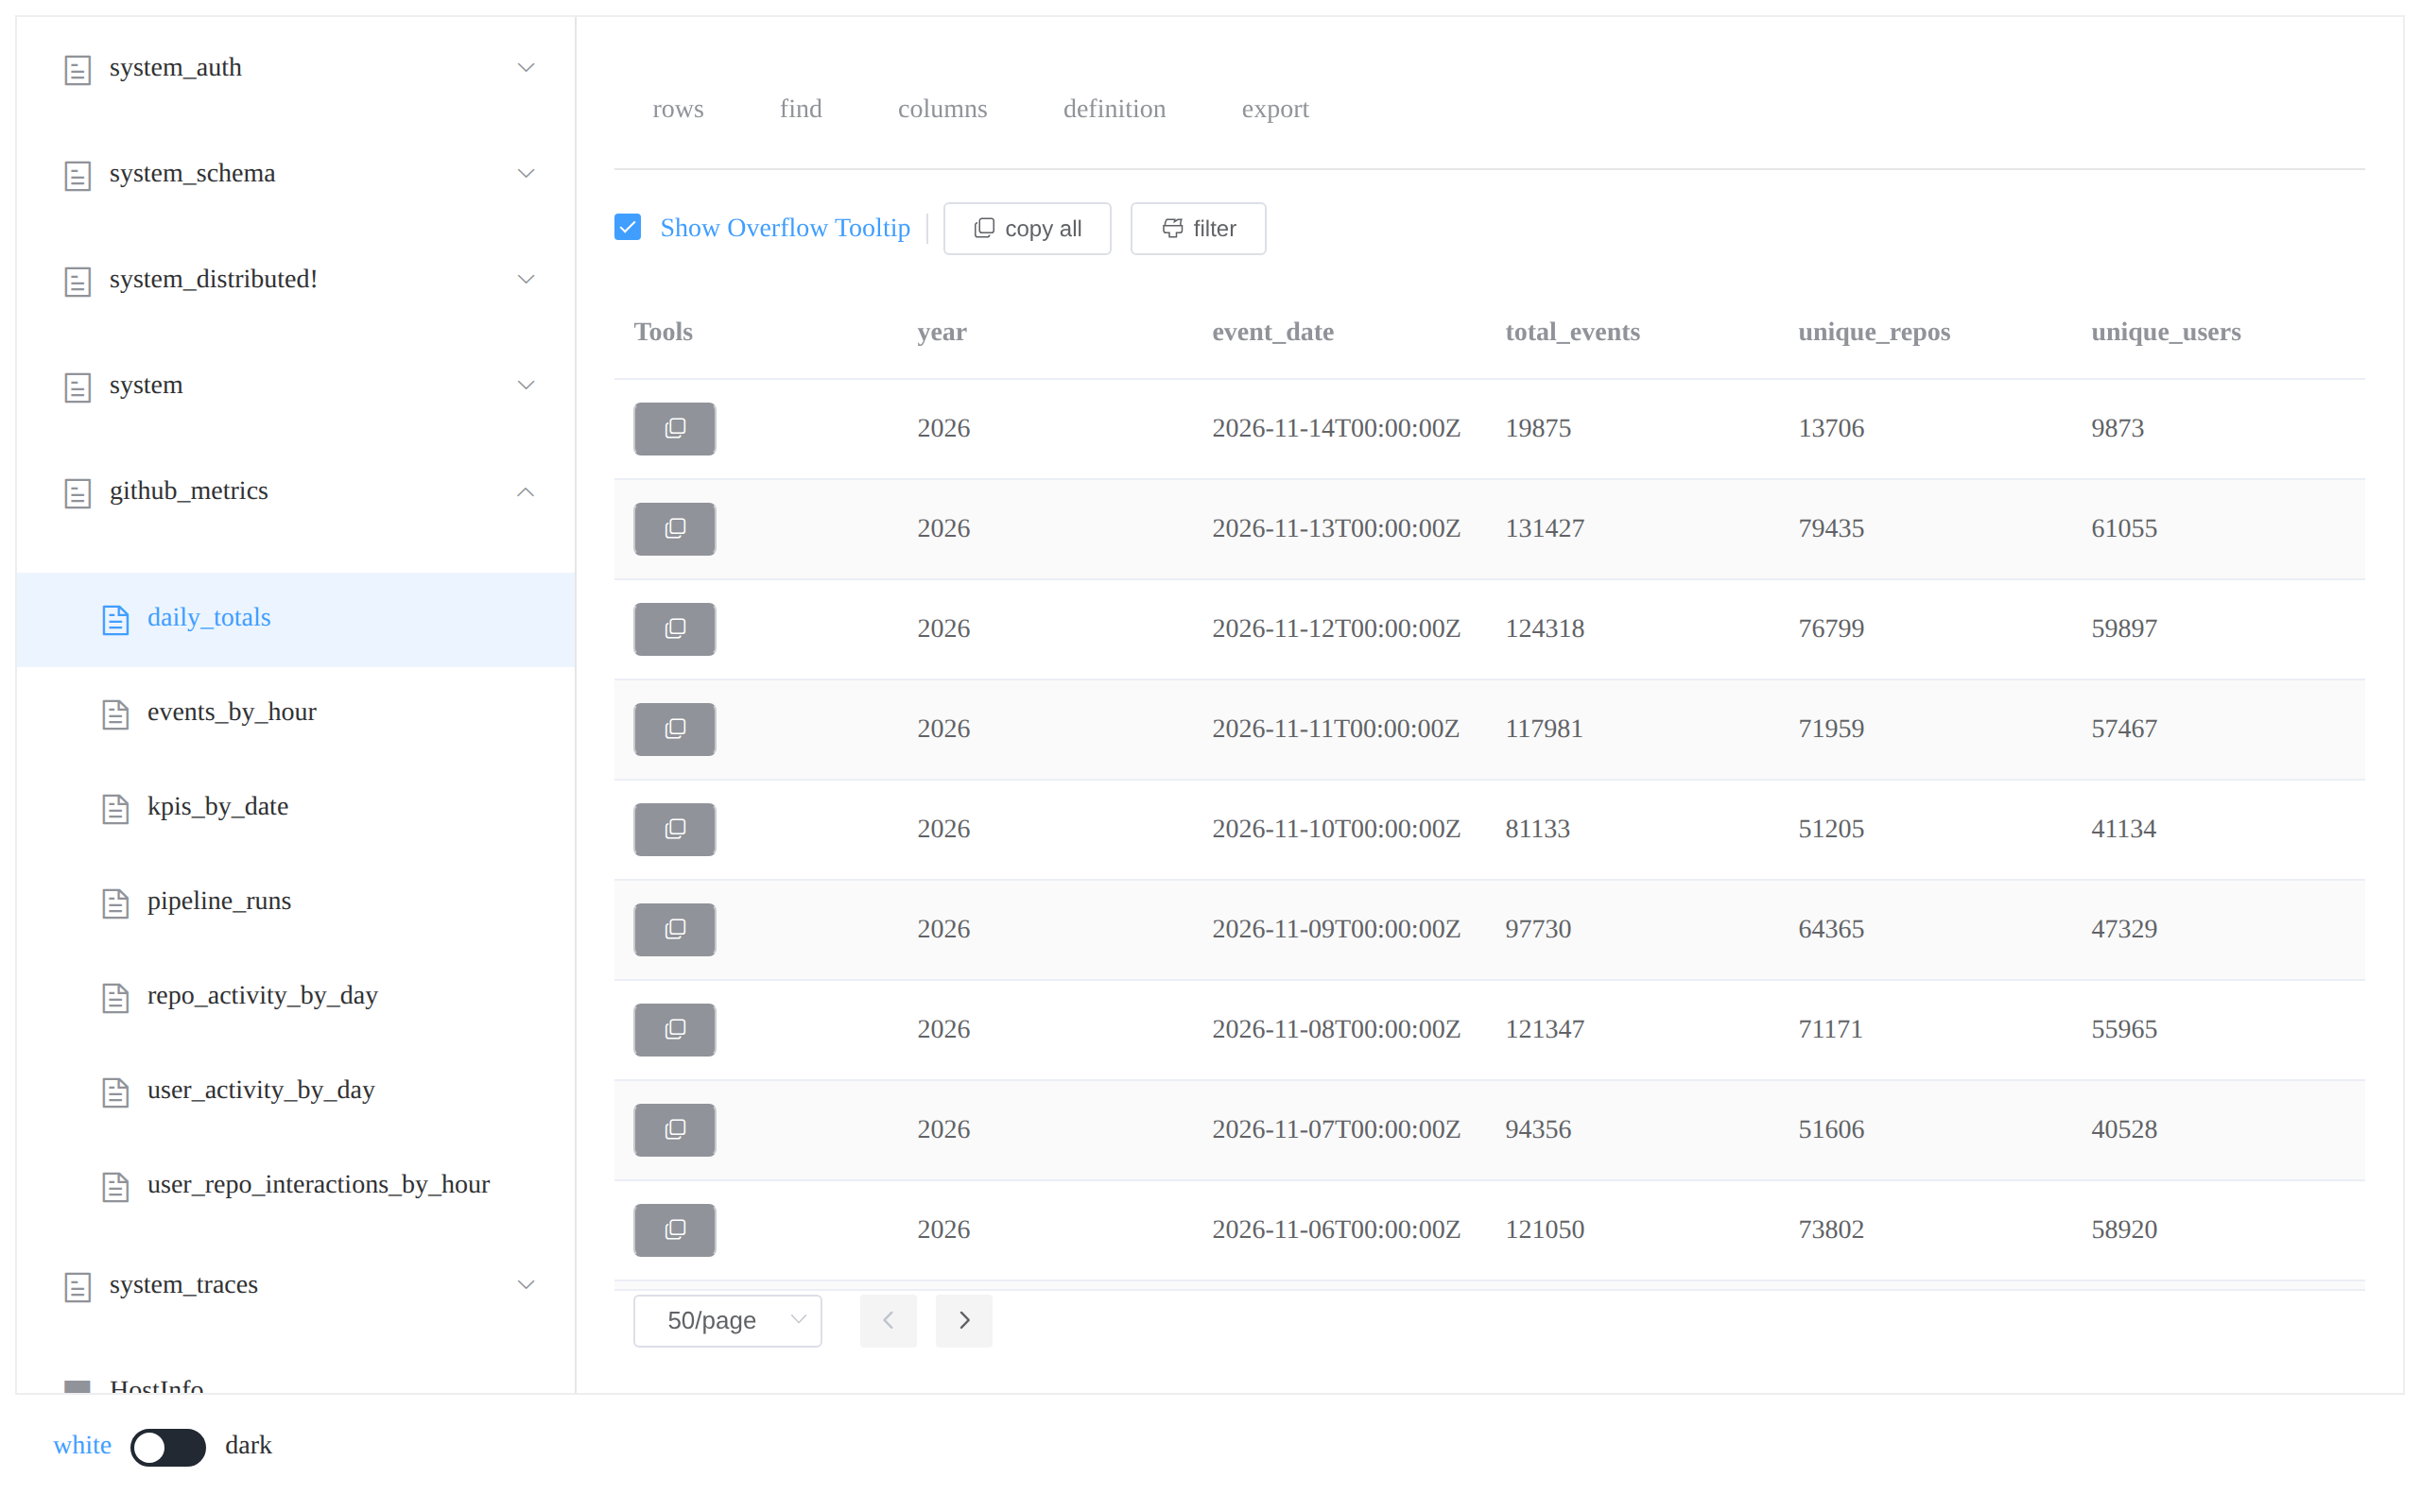
\includegraphics[width=0.93\textwidth]{db-cassandra-web.png}
    \caption{Tabla \texttt{daily\_totals} en Cassandra Web, capturada el 14 de noviembre. Cada fila resume un día: eventos, repositorios y usuarios distintos. La primera corresponde al día en curso, todavía parcial; las siguientes, a los últimos días completos del periodo.}
    \label{fig:db-cassandra-web}
\end{figure}

% ========================== MODELO DE NEO4J ==========================
\section{Modelo de Grafo en Neo4j}
\label{sec:neo4j}

Neo4j es la capa de \textbf{relaciones}. El grafo representa quién interactúa con qué repositorio y a qué organización pertenece cada repositorio. Las restricciones se crean con \repo{scripts/init_neo4j.cypher}{scripts/init\_neo4j.cypher}.

\subsection{Nodos y Relaciones}

\begin{figure}[H]
    \centering
    \begin{tikzpicture}[
        font=\small,
        nodo/.style={circle, draw=black, thick, minimum size=2.1cm, align=center},
        arrow/.style={-{Stealth[scale=1.2]}, thick},
        lbl/.style={font=\scriptsize, align=center, fill=white, inner sep=2pt}
    ]
    \node[nodo, fill=blue!14] (u) {\textbf{:User}\\ \texttt{login}};
    \node[nodo, fill=green!16, right=5.6cm of u] (r) {\textbf{:Repo}\\ \texttt{name}\\ \texttt{owner}};
    \node[nodo, fill=orange!20, right=3.6cm of r] (o) {\textbf{:Org}\\ \texttt{login}};
    \draw[arrow] (u) -- node[lbl] {\texttt{PUSHED} $|$ \texttt{OPENED\_PR} $|$ \texttt{OPENED\_ISSUE}\\ \texttt{STARRED} $|$ \texttt{FORKED}\\[0.2em] \{\texttt{count}, \texttt{first\_seen}, \texttt{last\_seen}\}} (r);
    \draw[arrow] (r) -- node[lbl] {\texttt{BELONGS\_TO}} (o);
    \end{tikzpicture}
    \caption{Modelo de grafo de propiedades: tres etiquetas de nodo y seis tipos de relación.}
    \label{fig:modelo-grafo}
\end{figure}

\begin{table}[H]
\centering
\caption{Elementos del grafo y su volumen al corte}
\label{tab:grafo}
\vspace{0.2cm}
\small
\begin{tabular}{@{}llp{5.6cm}r@{}}
\toprule
\textbf{Elemento} & \textbf{Tipo} & \textbf{Propiedades / origen} & \textbf{Cantidad} \\
\midrule
\texttt{:User}          & Nodo     & \texttt{login} (único)                            & 1,451,903 \\
\texttt{:Repo}          & Nodo     & \texttt{name} (único), \texttt{owner}             & 1,887,722 \\
\texttt{:Org}           & Nodo     & \texttt{login} (único)                            &   129,068 \\
\midrule
\texttt{PUSHED}         & Relación & \texttt{PushEvent}                                & 1,531,945 \\
\texttt{OPENED\_PR}     & Relación & \texttt{PullRequestEvent}                         &   654,560 \\
\texttt{STARRED}        & Relación & \texttt{WatchEvent}                               &   216,598 \\
\texttt{OPENED\_ISSUE}  & Relación & \texttt{IssuesEvent}                              &   175,188 \\
\texttt{FORKED}         & Relación & \texttt{ForkEvent}                                &    35,979 \\
\texttt{BELONGS\_TO}    & Relación & campo \texttt{org} del evento                     &   288,987 \\
\midrule
\multicolumn{3}{@{}l}{\textbf{Total de nodos}}      & \textbf{3,468,693} \\
\multicolumn{3}{@{}l}{\textbf{Total de relaciones}} & \textbf{2,903,257} \\
\bottomrule
\end{tabular}
\end{table}

Tres decisiones definen el modelo:

\begin{itemize}[leftmargin=*]
    \item \textbf{La relación agrega, no enumera.} Entre un usuario y un repositorio existe a lo sumo una relación de cada tipo, con la propiedad \texttt{count} acumulando cuántas veces ocurrió y \texttt{first\_seen}/\texttt{last\_seen} delimitando el periodo. Los 12.1 millones de \textit{pushes} con relación en el grafo se condensan así en 1.5 millones de aristas \texttt{PUSHED}. Modelar una arista por evento multiplicaría el tamaño del grafo sin aportar nada a las preguntas de conectividad.
    \item \textbf{El tipo de acción es el tipo de la relación.} Usar \texttt{PUSHED}, \texttt{STARRED}, etc.\ como tipos, en lugar de una relación genérica con una propiedad \texttt{tipo}, permite filtrar por tipo durante el recorrido sin leer propiedades.
    \item \textbf{Solo cinco tipos de evento generan relaciones.} Son los que expresan un vínculo directo de un usuario con un repositorio. Comentarios, revisiones y borrados no crean aristas.
\end{itemize}

\subsection{Restricciones}

Las tres restricciones de unicidad garantizan que no existan nodos duplicados y crean, a la vez, el índice que usa \texttt{MERGE} para localizar cada nodo:

\begin{lstlisting}[style=plano]
CREATE CONSTRAINT user_login IF NOT EXISTS FOR (u:User) REQUIRE u.login IS UNIQUE;
CREATE CONSTRAINT repo_name  IF NOT EXISTS FOR (r:Repo) REQUIRE r.name  IS UNIQUE;
CREATE CONSTRAINT org_login  IF NOT EXISTS FOR (o:Org)  REQUIRE o.login IS UNIQUE;
\end{lstlisting}

\subsection{Construcción del Grafo}

La etapa 5 (\repo{src/load_neo4j.py}{src/load\_neo4j.py}) no lee el archivo de origen ni MongoDB: lee la partición de la hora en la tabla \texttt{user\_repo\_\bk{}interactions\_\bk{}by\_hour} de Cassandra, agrupa las filas por tipo de relación y las envía en lotes de 1,000 con \texttt{UNWIND} y \texttt{MERGE}.

\bloque{Consulta de carga de relaciones (simplificada; el tipo de relación se sustituye por lote)}
\begin{lstlisting}[style=plano]
UNWIND $rows AS row
MERGE (u:User {login: row.user})
MERGE (r:Repo {name: row.repo})
  ON CREATE SET r.owner = split(row.repo, '/')[0]
MERGE (u)-[rel:PUSHED]->(r)
  ON CREATE SET rel.count = row.n,
                rel.first_seen = datetime(row.ts), rel.last_seen = datetime(row.ts)
  ON MATCH  SET rel.count = coalesce(rel.count, 0) + row.n,
                rel.last_seen = CASE WHEN datetime(row.ts) > rel.last_seen
                                     THEN datetime(row.ts) ELSE rel.last_seen END
\end{lstlisting}

\paragraph{Control de tamaño.} En cada hora solo entran al grafo los 10,000 repositorios y los 20,000 usuarios más activos de esa hora (parámetros \texttt{NEO4J\_TOP\_REPOS} y \texttt{NEO4J\_TOP\_USERS}). El grafo es, por tanto, una muestra sesgada hacia la actividad más intensa, lo que se declara en la metodología del \textit{dashboard}.

\paragraph{Idempotencia.} \texttt{MERGE} evita duplicar nodos y aristas, pero no evita sumar dos veces el \texttt{count}. Por eso la etapa consulta antes la columna \texttt{loaded\_neo4j} de \texttt{pipeline\_runs}: si la hora ya fue cargada en el grafo, se omite.

\paragraph{Reconstrucción.} Como el grafo se deriva íntegramente de Cassandra, puede regenerarse desde cero con \repo{scripts/rebuild_neo4j.py}{scripts/rebuild\_neo4j.py} sin volver a descargar ni a procesar los archivos de origen. Es la consecuencia práctica de la arquitectura por capas.

\subsection{Consultas de Grafo}

Las dos consultas siguientes ilustran por qué este dato reside en Neo4j. La primera es la base del KPI~5, que le añade un filtro por fecha sobre \texttt{first\_seen} (Sección~\ref{sec:kpis}); la segunda encuentra a los usuarios que comparten repositorios con uno dado, un recorrido de dos saltos.

\begin{lstlisting}[style=plano]
// Repositorios con más usuarios distintos conectados (grado del nodo)
MATCH (u:User)-[]->(r:Repo)
RETURN r.name AS repo, count(DISTINCT u) AS usuarios
ORDER BY usuarios DESC LIMIT 5;

// Usuarios que colaboran en los mismos repositorios que un usuario dado
MATCH (a:User {login: $login})-[]->(r:Repo)<-[]-(b:User)
WHERE a <> b
RETURN b.login AS colega, count(DISTINCT r) AS repos_en_comun
ORDER BY repos_en_comun DESC LIMIT 5;
\end{lstlisting}

\begin{table}[H]
\centering
\caption{Resultado de la primera consulta sobre el grafo acumulado}
\label{tab:top-repos}
\vspace{0.2cm}
\small
\begin{tabular}{@{}lr@{}}
\toprule
\textbf{Repositorio} & \textbf{Usuarios distintos conectados} \\
\midrule
\texttt{morluto/rea}                     & 6,843 \\
\texttt{storytold/photocraft}            & 1,483 \\
\texttt{Ebony-Vinyl/dsh-our-free-model}  & 1,148 \\
\texttt{boykopovar/AnyPS5}               & 1,025 \\
\texttt{debpalash/VoiceStudio}           &   842 \\
\bottomrule
\end{tabular}
\end{table}

El primer repositorio cuadruplica al segundo. El grafo permite ir más allá del número, porque conserva el tipo de cada relación (Tabla~\ref{tab:morluto}).

\begin{table}[H]
\centering
\caption{Relaciones entrantes de \texttt{morluto/rea} por tipo}
\label{tab:morluto}
\vspace{0.2cm}
\small
\begin{tabular}{@{}lrr@{}}
\toprule
\textbf{Tipo de relación} & \textbf{Relaciones} & \textbf{Interacciones (\texttt{count})} \\
\midrule
\texttt{STARRED}       & 5,628 & 5,630 \\
\texttt{FORKED}        & 1,156 & 1,156 \\
\texttt{OPENED\_PR}    &    58 &   143 \\
\texttt{OPENED\_ISSUE} &    26 &   173 \\
\texttt{PUSHED}        &     7 &   410 \\
\bottomrule
\end{tabular}
\end{table}

El 82\,\% de los usuarios conectados (5,608) tiene como única relación una estrella, y la actividad de código se reduce a 7 cuentas que hicieron \textit{push}. Un grado alto no implica por sí solo una comunidad de colaboradores: aquí describe popularidad, no colaboración, y esa distinción solo es visible al examinar el tipo de las relaciones. El vecindario se explora de forma interactiva en el \textit{dashboard} (Figura~\ref{fig:dash-neo4j-vecindario}).

% ============================ DAG DE AIRFLOW =========================
\section{Explicación del DAG de Airflow}
\label{sec:airflow}

La automatización se implementa en un único DAG, \texttt{github\_events\_pipeline}, definido en \repo{dags/github_events_dag.py}{dags/github\_events\_dag.py}. Contiene las seis etapas que exige el enunciado, encadenadas linealmente, y se ejecuta de forma programada cada hora.

\begin{figure}[H]
    \centering
    \begin{tikzpicture}[
        font=\scriptsize,
        task/.style={rectangle, draw=black, thick, rounded corners=2pt, minimum width=2.15cm, minimum height=1.25cm, align=center},
        arrow/.style={-{Stealth[scale=1.0]}, thick}
    ]
    \node[task, fill=gray!12] (t1) {\textbf{1}\\ \texttt{extract\_data}};
    \node[task, fill=gray!12, right=0.32cm of t1] (t2) {\textbf{2}\\ \texttt{validate\_}\\ \texttt{and\_clean}};
    \node[task, fill=green!16, right=0.32cm of t2] (t3) {\textbf{3}\\ \texttt{load\_mongodb}};
    \node[task, fill=blue!14, right=0.32cm of t3] (t4) {\textbf{4}\\ \texttt{transform\_load\_}\\ \texttt{cassandra}};
    \node[task, fill=violet!16, right=0.32cm of t4] (t5) {\textbf{5}\\ \texttt{build\_graph\_}\\ \texttt{neo4j}};
    \node[task, fill=orange!16, right=0.32cm of t5] (t6) {\textbf{6}\\ \texttt{generate\_kpis}};
    \draw[arrow] (t1) -- (t2); \draw[arrow] (t2) -- (t3); \draw[arrow] (t3) -- (t4);
    \draw[arrow] (t4) -- (t5); \draw[arrow] (t5) -- (t6);
    \end{tikzpicture}
    \caption{Tareas del DAG \texttt{github\_events\_pipeline} y su orden de ejecución.}
    \label{fig:dag}
\end{figure}

\subsection{Etapas}

Cada tarea es un \texttt{PythonOperator} que invoca una función del paquete \texttt{src/}. La lógica vive fuera del DAG para que los mismos módulos puedan ejecutarse desde la carga histórica y desde los \textit{notebooks}.

\begin{table}[H]
\centering
\caption{Etapas del DAG: qué lee y qué escribe cada una}
\label{tab:etapas}
\vspace{0.2cm}
\footnotesize
\begin{tabular}{@{}cp{3.3cm}p{4.9cm}p{5.4cm}@{}}
\toprule
\textbf{\#} & \textbf{Tarea} & \textbf{Lee} & \textbf{Escribe} \\
\midrule
1 & \texttt{extract\_data} &
Archivo horario de GH Archive (HTTP). &
\texttt{data/raw/AAAA-MM-DD-H.json.gz}. Si ya existe, no lo vuelve a descargar. \\
\addlinespace
2 & \texttt{validate\_and\_clean} &
Archivo crudo, línea a línea, sin cargarlo entero en memoria. &
Archivo intermedio JSONL con los eventos válidos, y estadísticas de calidad (crudos, válidos, duplicados, rechazados y motivos). \\
\addlinespace
3 & \texttt{load\_mongodb} &
Archivo intermedio. &
Colección \texttt{events} (\textit{upsert} por \texttt{\_id}) y un documento en \texttt{ingestion\_log}. \\
\addlinespace
4 & \texttt{transform\_load\_\bk{}cassandra} &
\textbf{MongoDB}: eventos de la hora, por el índice de \texttt{created\_at}. &
Cinco tablas de agregados de Cassandra y la fila de la hora en \texttt{pipeline\_runs}. \\
\addlinespace
5 & \texttt{build\_graph\_neo4j} &
\textbf{Cassandra}: partición de la hora en \texttt{user\_repo\_\bk{}interactions\_\bk{}by\_hour}. &
Nodos y relaciones en Neo4j (\texttt{MERGE}); marca \texttt{loaded\_neo4j} en \texttt{pipeline\_runs}. \\
\addlinespace
6 & \texttt{generate\_kpis} &
\textbf{Las tres bases}: Cassandra (KPI 1--3), MongoDB (KPI 4), Neo4j (KPI 5). &
Cinco filas en \texttt{kpis\_by\_date} para el día de la hora procesada. \\
\bottomrule
\end{tabular}
\end{table}

Las tareas se comunican por XCom, pero \textbf{solo intercambian metadatos}: el nombre y la ruta del archivo, la hora procesada y las estadísticas de cada etapa. Los eventos nunca viajan por XCom; cada etapa los lee de la capa de almacenamiento anterior. Esto mantiene pequeña la base de metadatos de Airflow y hace que cada etapa sea reejecutable de forma independiente.

\subsection{Programación}

\begin{table}[H]
\centering
\caption{Parámetros de programación y tolerancia a fallos del DAG}
\label{tab:dag-params}
\vspace{0.2cm}
\small
\begin{tabular}{@{}llp{7.6cm}@{}}
\toprule
\textbf{Parámetro} & \textbf{Valor} & \textbf{Efecto} \\
\midrule
\texttt{schedule}           & \texttt{@hourly}  & Una corrida al inicio de cada hora. \\
\texttt{catchup}            & \texttt{False}    & No repone corridas pasadas al activar el DAG; el pasado se carga con el \textit{script} de carga histórica. \\
\texttt{max\_active\_runs}  & 1                 & Nunca hay dos corridas simultáneas, lo que protege las tablas diarias de Cassandra, que se actualizan leyendo y reescribiendo. \\
\texttt{retries}            & 3                 & Reintentos automáticos por tarea. \\
\texttt{retry\_delay}       & 5 minutos         & Espera entre reintentos; cubre el caso de que el archivo de la hora aún no esté publicado. \\
Ejecutor                    & \texttt{LocalExecutor} & Las tareas corren como procesos del planificador. \\
\bottomrule
\end{tabular}
\end{table}

Cada corrida procesa la hora \texttt{data\_interval\_start} $-$ 2\,h. El retraso de dos horas absorbe la demora con la que GH Archive publica cada archivo; así, la corrida programada a las 05:00 UTC procesa el archivo de las 02:00 UTC.

\subsection{Idempotencia}

Un flujo programado debe poder reintentarse sin alterar el resultado. Cada etapa lo garantiza con el mecanismo propio de su base de datos:

\begin{itemize}[leftmargin=*]
    \item \textbf{Extracción:} descarga a un archivo temporal y lo renombra al terminar; si el destino ya existe, no descarga.
    \item \textbf{MongoDB:} \textit{upsert} con \texttt{\$setOnInsert} sobre el \texttt{\_id} del evento.
    \item \textbf{Cassandra:} la etapa se omite si la hora ya figura en \texttt{pipeline\_runs}.
    \item \textbf{Neo4j:} la etapa se omite si \texttt{pipeline\_runs.loaded\_neo4j} es mayor que cero para esa hora.
    \item \textbf{Indicadores:} se recalculan completos y se sobrescriben por clave primaria (día, indicador).
\end{itemize}

\subsection{Evidencia de Ejecución}

\begin{figure}[H]
    \centering
    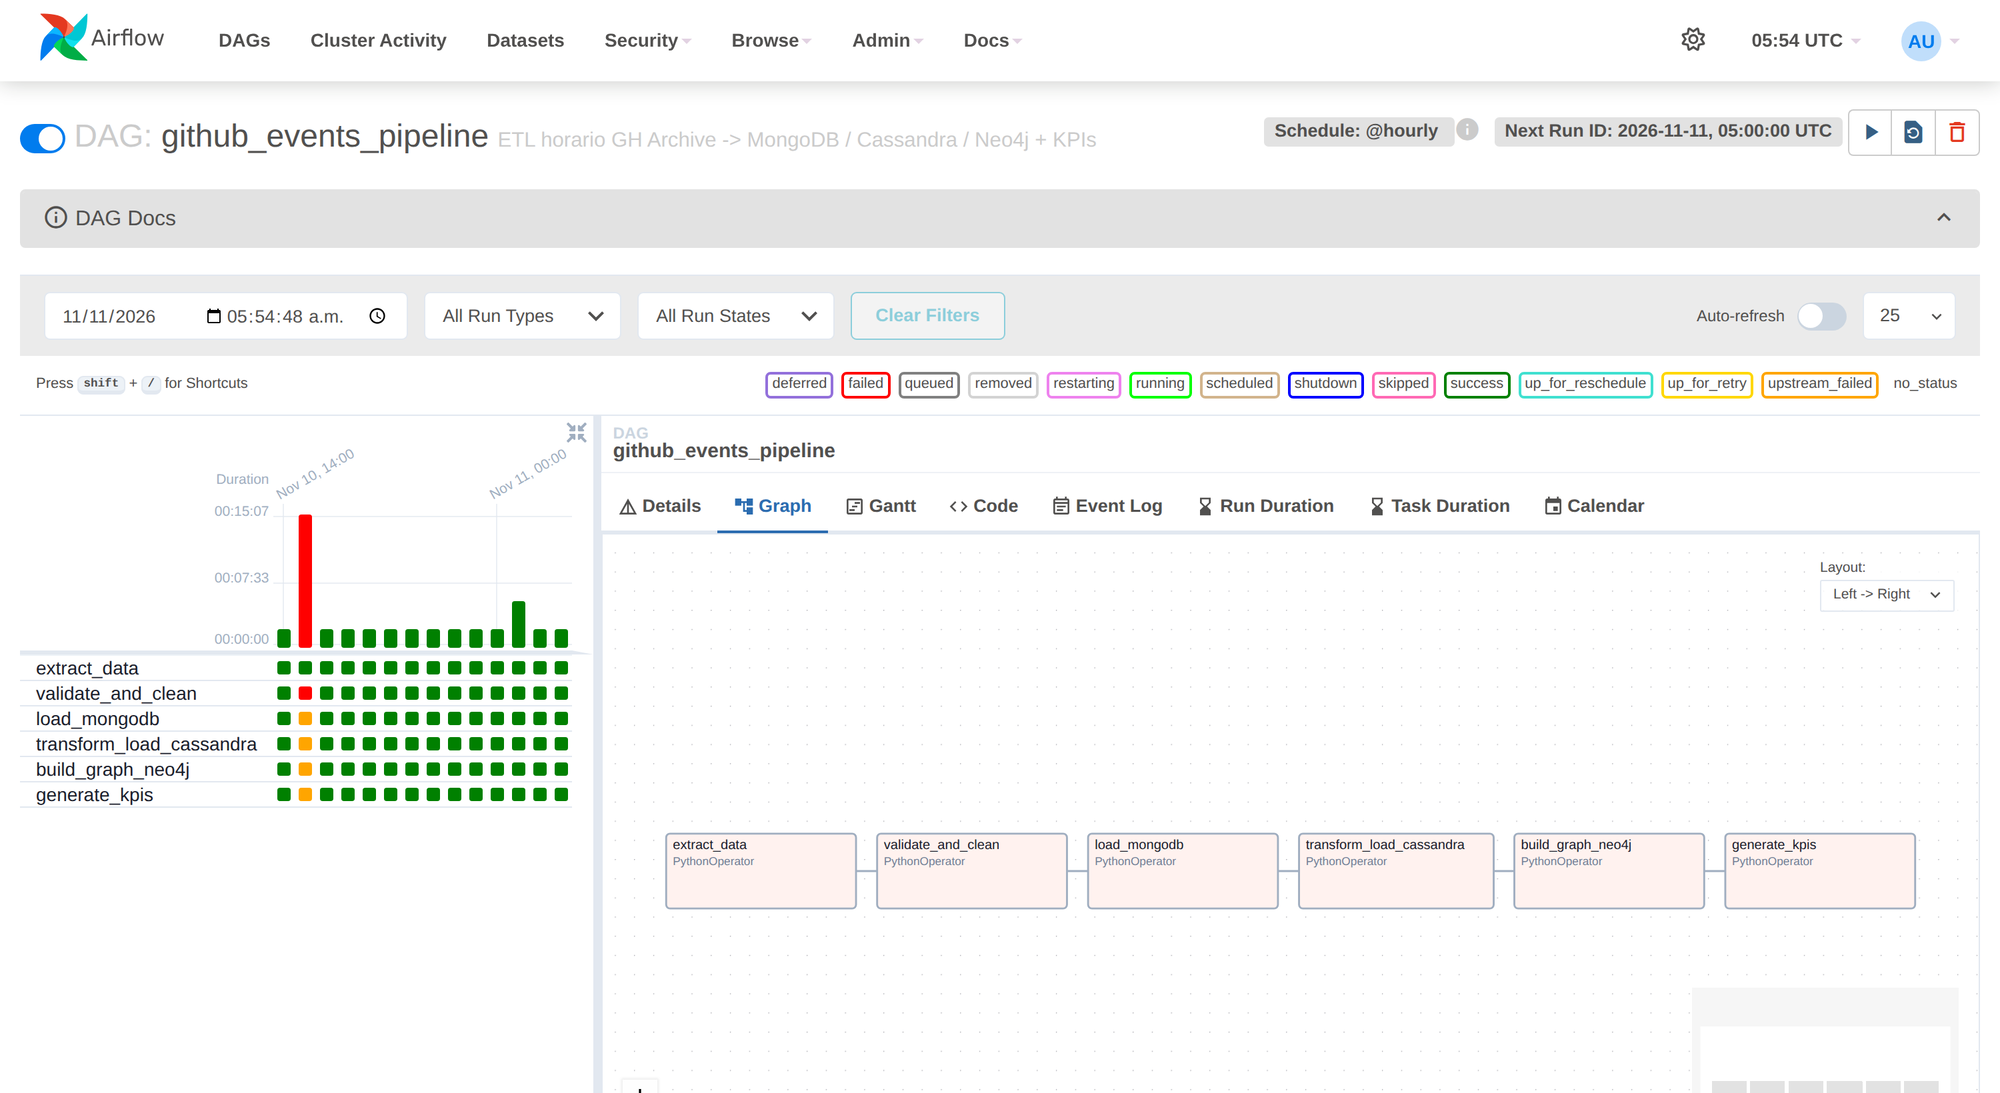
\includegraphics[width=\textwidth]{airflow-grafo.png}
    \caption{Interfaz de Airflow: DAG activo con programación \texttt{@hourly}. A la izquierda, el historial de corridas por tarea; a la derecha, el grafo de las seis tareas.}
    \label{fig:airflow-grafo}
\end{figure}

Desde su activación, el 10 de noviembre de 2026 a las 14:36 UTC, hasta la captura de la Figura~\ref{fig:airflow-grafo}, el DAG registró 14 corridas: 13 exitosas y 1 fallida. Una corrida normal sobre una hora de noviembre (unos 3,500 eventos) completa las seis etapas en un tiempo de entre 7 y 21 segundos.

\subsection{Diagnóstico de la Corrida Fallida}
\label{subsec:fallo}

La corrida programada para las 14:00 UTC del 10 de noviembre falló en la tarea \texttt{validate\_and\_clean} tras agotar sus tres intentos (15:00, 15:05 y 15:10 UTC). El registro de la tarea muestra el mismo error en los tres:

\begin{lstlisting}[style=plano]
PermissionError: [Errno 13] Permission denied:
    '/opt/airflow/data/processed/2026-11-10-12.clean.jsonl'
\end{lstlisting}

\paragraph{Causa.} El error no tiene relación con los datos. La carpeta \texttt{data/} está montada a la vez en el contenedor de Airflow, cuyos procesos corren con el identificador de usuario 50000, y en el de Jupyter, que usa el 1000. La hora 12 de ese día ya había sido procesada por la carga histórica lanzada desde Jupyter, que reescribió el archivo intermedio a las 14:44 UTC, dieciséis minutos antes de la corrida; el archivo existía y pertenecía al usuario 1000. Al intentar abrirlo para sobrescribirlo, Airflow no tenía permiso de escritura sobre él. El listado de la carpeta lo confirma: los archivos de las horas 10 y 12 pertenecen al usuario 1000, y los de las horas 11 y 13, al 50000.

\paragraph{Impacto.} Ninguno sobre los datos: la hora 12 figura en \texttt{pipeline\_runs} con sus 3,778 eventos, registrada a las 14:36 UTC, antes de la corrida fallida, que por tanto habría sido redundante.

\paragraph{Corrección.} La escritura del archivo intermedio se cambió a una \textbf{escritura atómica}: se escribe en un archivo temporal propio del proceso y se reemplaza el destino con \texttt{os.replace}. Reemplazar una entrada de directorio solo requiere permiso sobre la carpeta, no sobre el archivo previo, por lo que el conflicto desaparece; además, un proceso interrumpido ya no puede dejar un archivo intermedio a medio escribir.

\paragraph{Una segunda observación.} En \texttt{pipeline\_runs} faltan dos horas consecutivas: las 23:00 UTC del 10 de noviembre y las 00:00 UTC del 11. Corresponden a las corridas de las 01:00 y 02:00 UTC del día 11, que nunca se crearon porque el planificador no estuvo activo en ese intervalo (la corrida de las 00:00 UTC comenzó recién a las 04:49 UTC). Con \texttt{catchup=False} Airflow no repone esas corridas al reanudar. No es una pérdida de datos, puesto que los archivos siguen publicados en la fuente y el \textit{script} de carga histórica los incorpora, pero ilustra el costo de esa configuración: la continuidad depende de que el planificador no se detenga. El \textit{dashboard} hace visible la brecha al marcar el 10 de noviembre como día parcial, con 23 de 24 horas.

% ========================== OPERACIONES CRUD =========================
\section{Operaciones CRUD}
\label{sec:crud}

Las cuatro operaciones básicas se implementaron sobre cada base de datos en un \textit{notebook} propio, pensado para ejecutarse celda a celda durante la exposición. Los tres siguen el mismo guion: crear un registro de demostración claramente identificable, consultarlo, modificarlo, eliminarlo y comprobar que ya no existe, de manera que la demostración no altera los datos reales.

\begin{table}[H]
\centering
\caption{Operaciones CRUD implementadas por base de datos}
\label{tab:crud}
\vspace{0.2cm}
\footnotesize
\begin{tabular}{@{}p{1.6cm}>{\raggedright\arraybackslash}p{4.1cm}>{\raggedright\arraybackslash}p{4.1cm}>{\raggedright\arraybackslash}p{4.3cm}@{}}
\toprule
\textbf{Operación} & \textbf{MongoDB} & \textbf{Cassandra} & \textbf{Neo4j} \\
\midrule
Crear &
\texttt{insert\_one} de un evento de prueba &
\texttt{INSERT} de dos filas en un día ficticio &
\texttt{MERGE} de un usuario, un repositorio y la relación \texttt{STARRED} \\
\addlinespace
Consultar &
\texttt{find\_one} por \texttt{\_id}; \texttt{find} con filtro, proyección y orden; \texttt{aggregate} por tipo &
\texttt{SELECT} por clave de partición; lectura de indicadores del último día &
\texttt{MATCH} del patrón; grado por repositorio; colaboradores a dos saltos \\
\addlinespace
Actualizar &
\texttt{update\_one} con \texttt{\$set} sobre un campo anidado y \texttt{\$inc} &
\texttt{UPDATE} de un contador por clave primaria completa &
\texttt{SET} sobre una propiedad de la relación y otra del nodo \\
\addlinespace
Eliminar &
\texttt{delete\_one} y verificación &
\texttt{DELETE} de una fila y de la partición completa &
\texttt{DELETE} de la relación y \texttt{DETACH DELETE} de los nodos \\
\midrule
\textit{Notebook} &
\repo{notebooks/02_crud_mongodb.ipynb}{02\_crud\_\bk{}mongodb.ipynb} &
\repo{notebooks/03_crud_cassandra.ipynb}{03\_crud\_\bk{}cassandra.ipynb} &
\repo{notebooks/04_crud_neo4j.ipynb}{04\_crud\_\bk{}neo4j.ipynb} \\
\bottomrule
\end{tabular}
\end{table}

\subsection{MongoDB}

\begin{lstlisting}[style=py]
# C - crear
doc = {'_id': demo_id, 'type': 'WatchEvent',
       'actor': {'id': 1, 'login': 'estudiante_utec'},
       'repo': {'id': 1, 'name': 'utec/bigdata-demo'}, 'public': True,
       'created_at': datetime.now(timezone.utc), 'payload': {'action': 'started'}}
col.insert_one(doc)

# R - consultar: por clave, y con filtro + proyección + orden
col.find_one({'_id': demo_id})
col.find({'type': 'PushEvent'}, {'actor.login': 1, 'repo.name': 1, 'created_at': 1}) \
   .sort('created_at', -1).limit(5)

# U - actualizar un campo anidado y un contador
col.update_one({'_id': demo_id},
               {'$set': {'payload.action': 'stopped', 'revisado': True},
                '$inc': {'veces_editado': 1}})

# D - eliminar
col.delete_one({'_id': demo_id})
\end{lstlisting}

La actualización ilustra la flexibilidad del modelo documental: añade al documento dos campos (\texttt{revisado}, \texttt{veces\_editado}) que no existían en ningún otro, sin modificar esquema alguno.

\subsection{Cassandra}

\begin{lstlisting}[style=py]
demo_day = date(2099, 1, 1)      # día ficticio: no se mezcla con datos reales

# C - insertar
s.execute('INSERT INTO events_by_hour (event_date, event_hour, event_type, event_count) '
          'VALUES (%s,%s,%s,%s)', (demo_day, 10, 'PushEvent', 123))

# R - consultar una partición completa
s.execute('SELECT * FROM events_by_hour WHERE event_date=%s', (demo_day,))

# U - actualizar (exige la clave primaria completa)
s.execute('UPDATE events_by_hour SET event_count=%s '
          'WHERE event_date=%s AND event_hour=%s AND event_type=%s',
          (999, demo_day, 10, 'PushEvent'))

# D - eliminar una fila y, después, la partición entera
s.execute('DELETE FROM events_by_hour WHERE event_date=%s AND event_hour=%s AND event_type=%s',
          (demo_day, 10, 'PushEvent'))
s.execute('DELETE FROM events_by_hour WHERE event_date=%s', (demo_day,))
\end{lstlisting}

Dos particularidades de Cassandra quedan a la vista. Toda consulta debe indicar la clave de partición, lo que obliga a conocer de antemano por dónde se va a leer. Y \texttt{INSERT} y \texttt{UPDATE} son, en la práctica, la misma operación de escritura: ambos sobrescriben la celda identificada por la clave primaria.

\subsection{Neo4j}

\begin{lstlisting}[style=plano]
// C - crear dos nodos y la relación entre ellos
MERGE (u:User {login:'estudiante_utec'})
MERGE (r:Repo {name:'utec/bigdata-demo'})
MERGE (u)-[rel:STARRED]->(r)
  SET rel.count = 1, rel.first_seen = datetime()

// R - consultar el patrón
MATCH (u:User {login:'estudiante_utec'})-[rel]->(r:Repo)
RETURN u.login, type(rel), rel.count, r.name

// U - actualizar una propiedad de la relación y otra del nodo
MATCH (u:User {login:'estudiante_utec'})-[rel:STARRED]->(r:Repo {name:'utec/bigdata-demo'})
  SET rel.count = rel.count + 1, u.rol = 'estudiante'

// D - eliminar la relación y luego los nodos
MATCH (:User {login:'estudiante_utec'})-[rel:STARRED]->(:Repo {name:'utec/bigdata-demo'})
DELETE rel
MATCH (n) WHERE n.login = 'estudiante_utec' OR n.name = 'utec/bigdata-demo'
DETACH DELETE n
\end{lstlisting}

El \textit{notebook} cubre los cuatro casos que pide el enunciado para Neo4j: crear nodo, crear relación, actualizar propiedades (tanto de la relación como del nodo) y eliminar relaciones y nodos.

% ========================= KPIs IMPLEMENTADOS ========================
\section{KPIs Implementados}
\label{sec:kpis}

Se definieron cinco indicadores, con la condición de que \textbf{cada base de datos aporte al menos uno}: tres se calculan desde Cassandra, uno desde MongoDB y uno desde Neo4j. La etapa 6 del DAG (\repo{src/kpis.py}{src/kpis.py}) los recalcula en cada corrida para el día de la hora procesada y los guarda en la tabla \texttt{kpis\_by\_date}, de donde los lee el \textit{dashboard}.

\begin{table}[H]
\centering
\caption{Resumen de los cinco indicadores y su valor para el lunes 12 de octubre de 2026}
\label{tab:kpis}
\vspace{0.2cm}
\footnotesize
\begin{tabular}{@{}clllr@{}}
\toprule
\textbf{KPI} & \textbf{Indicador} & \textbf{Base de datos} & \textbf{Fuente} & \textbf{Valor (12 oct)} \\
\midrule
1 & Eventos procesados por día       & Cassandra & \texttt{events\_by\_hour}          & 1,981,972 \\
2 & Crecimiento diario (flujo estable) & Cassandra & \texttt{events\_by\_hour}          & $-14.0$\,\% \\
3 & Actividad por usuario & Cassandra & \texttt{daily\_totals}            & 4.07 \\
4 & Tasa de fusión de PR & MongoDB & \texttt{payload.action}       & 93.8\,\% \\
5 & Repositorio más conectado        & Neo4j     & grado de \texttt{:Repo}       & 2,034 usuarios \\
\bottomrule
\end{tabular}
\end{table}

Los valores de ejemplo corresponden al 12 de octubre, un día con las 24 horas cargadas y con el flujo de referencias de Git completo. Para cada indicador se presenta su definición, su fórmula de cálculo y su interpretación, como exige el enunciado, seguidas de la ficha correspondiente del \textit{dashboard}.

% ------------------------------------------------------------------ KPI 1
\subsection{KPI 1: Número de Eventos Procesados por Día}

\paragraph{Definición.} Cantidad de eventos públicos de GitHub procesados por el \textit{pipeline} en el día $D$ (UTC).

\paragraph{Fórmula.}
\[
E_D \;=\; \sum_{h \,\in\, H_D} \; \sum_{t} \; n_{D,h,t}
\]
donde $n_{D,h,t}$ es el número de eventos del tipo $t$ en la hora $h$ del día $D$ (una fila de \texttt{events\_by\_hour}) y $H_D$ es el conjunto de horas cargadas de ese día.

\paragraph{Interpretación.} Mide el volumen de actividad ingerido y es la base de los demás indicadores. Solo es comparable entre días con las mismas horas cargadas y, como se mostró en la Sección~\ref{subsec:cobertura}, entre días con la misma cobertura de la fuente. Por eso la etapa 6 guarda junto al valor dos datos de contexto, que el \textit{dashboard} muestra en la tarjeta del indicador: los eventos del flujo estable y el número de horas del día que traen \textit{push}.

\paragraph{Valor.} $E_D = 1{,}981{,}972$ eventos el 12 de octubre, un 176\,\% por encima de la media de los 44 días completos (718,507). De ellos, 71,580 pertenecen al flujo estable, y el flujo de referencias de Git estuvo presente en las 24 horas.

\captura{dash-kpi1.png}{Ficha del KPI 1 en el \textit{dashboard}: definición, fórmula, cálculo para la fecha, lectura y evolución en el periodo.}

% ------------------------------------------------------------------ KPI 2
\subsection{KPI 2: Crecimiento Diario de Eventos}

\paragraph{Definición.} Variación porcentual, respecto al día anterior, del volumen de eventos del \textbf{flujo estable} (todos los tipos excepto \texttt{PushEvent}, \texttt{CreateEvent} y \texttt{DeleteEvent}), calculada sobre las horas cargadas en ambos días.

\paragraph{Fórmula.}
\[
G_D \;=\; \frac{S_D(H) - S_{D-1}(H)}{S_{D-1}(H)} \times 100,
\qquad S_D(H) \;=\; \sum_{h \,\in\, H} \; \sum_{t \,\notin\, I} n_{D,h,t},
\qquad H \;=\; H_D \cap H_{D-1}
\]
donde $I$ es el conjunto de los tres tipos intermitentes y $S_D(H)$ son los eventos del flujo estable del día $D$ sumando únicamente las horas de $H$. Si no hay datos del día anterior, el indicador no se calcula.

\paragraph{Interpretación.} $G_D > 0$ indica que la actividad de colaboración crece y $G_D < 0$ que disminuye. Al excluir los tipos intermitentes, un hueco de cobertura de la fuente no se lee como una caída ni como una subida de actividad.

\paragraph{Valor.} $G_D = (71{,}580 - 83{,}258) / 83{,}258 \times 100 = -14.0$\,\% frente al domingo 11 de octubre, sobre las mismas 24 horas. Con todos los tipos, ese mismo día habría marcado $+17.9$\,\%: el volumen total subió porque la fuente entregó más \textit{pushes}, mientras la actividad de colaboración bajaba.

\paragraph{Decisión de diseño.} El indicador pasó por dos correcciones. La primera versión comparaba totales diarios: un día a medio procesar aparecía con variaciones ficticias de más de 100 puntos, y el primer día del periodo mostraba un engañoso 0\,\%. Restringir la comparación a las horas comunes y dejar el valor nulo cuando no hay día previo eliminó ambos artefactos. La segunda corrección responde al hallazgo de la Sección~\ref{subsec:cobertura}. Con todos los tipos de evento, el indicador oscilaba entre $-92.6$\,\% y $+448.4$\,\%, y sus extremos coincidían con los días en que el flujo de referencias de Git aparecía o desaparecía de la fuente: el 7 de octubre marcaba $-89.2$\,\% cuando el flujo estable de ese día en realidad creció un 34.4\,\%, y el 25 de octubre marcaba $+169.5$\,\% con el flujo estable cayendo un 18.8\,\%. Calculado sobre el flujo estable, el indicador se mueve entre $-44.5$\,\% y $+57.4$\,\% en todo el periodo. Como Cassandra conserva los conteos por hora y tipo, el cambio no exigió recargar datos: los indicadores de los 44 días se recalcularon con \repo{scripts/recompute_kpis.py}{scripts/recompute\_kpis.py}.

\captura{dash-kpi2.png}{Ficha del KPI 2. Al calcularse sobre el flujo estable, la serie ya no reproduce los escalones de cobertura de la fuente.}

% ------------------------------------------------------------------ KPI 3
\subsection{KPI 3: Promedio de Actividad por Usuario}

\paragraph{Definición.} Promedio de eventos generados por cada usuario activo (actor distinto) en el día.

\paragraph{Fórmula.}
\[
A_D \;=\; \frac{E_D}{U_D}
\]
donde $U_D$ es el número de usuarios distintos del día (\texttt{daily\_totals.unique\_users}).

\paragraph{Interpretación.} Mide la intensidad de uso. Como la distribución de actividad es muy asimétrica, describe la intensidad agregada y no al usuario típico.

\paragraph{Valor.} $A_D = 1{,}981{,}972 / 486{,}477 = 4.07$ eventos por usuario. La cifra convive con una mediana de 1 evento por usuario: el 1\,\% de las cuentas más activas concentra el 43.4\,\% de los eventos del día, y las 4,019 cuentas automatizadas (sufijo \texttt{[bot]}) generan el 21.7\,\%. Una sola de ellas, \texttt{github-actions[bot]}, aporta 309,389 eventos, el 15.6\,\% del total.

\captura{dash-kpi3.png}{Ficha del KPI 3.}

% ------------------------------------------------------------------ KPI 4
\subsection{KPI 4: Tasa de Fusión de \textit{Pull Requests}}

\paragraph{Definición.} Porcentaje de los \textit{pull requests} cerrados en el día que fueron fusionados (aceptados).

\paragraph{Fórmula.}
\[
T_D \;=\; \frac{F_D}{F_D + N_D} \times 100
\]
donde $F_D$ es el número de eventos \texttt{PullRequestEvent} del día con \texttt{payload.action = "merged"} y $N_D$ el de aquellos con \texttt{payload.action = "closed"} (cerrados sin fusionar).

\paragraph{Interpretación.} Indica qué proporción del trabajo que se somete a revisión termina aceptada; es una medida de la salud del flujo de contribución.

\paragraph{Valor.} $T_D = 8{,}314 / (8{,}314 + 545) \times 100 = 93.8$\,\%. En todo el periodo se mantiene entre 88.8\,\% y 94.9\,\%, con media de 93.4\,\%.

\paragraph{Por qué MongoDB.} Es el único indicador que requiere un campo del \texttt{payload}. Cassandra solo conserva conteos por tipo de evento y no distingue un \textit{pull request} abierto de uno fusionado. La agregación se apoya en el índice \texttt{ix\_type\_date}:

\begin{lstlisting}[style=plano]
db.events.aggregate([
  { $match: { type: "PullRequestEvent",
              created_at: { $gte: ISODate("2026-10-12T00:00:00Z"),
                            $lt:  ISODate("2026-10-13T00:00:00Z") } } },
  { $group: { _id: "$payload.action", n: { $sum: 1 } } }
])
\end{lstlisting}

\captura{dash-kpi4.png}{Ficha del KPI 4. Es el indicador más estable del periodo porque depende del flujo de colaboración, cuya cobertura no varía.}

% ------------------------------------------------------------------ KPI 5
\subsection{KPI 5: Repositorio con Mayor Número de Conexiones}

\paragraph{Definición.} Repositorio con más usuarios distintos conectados en el grafo acumulado hasta el final del día $D$, es decir, el nodo \texttt{Repo} de mayor grado de entrada considerando solo las relaciones cuya primera interacción ocurrió hasta ese día.

\paragraph{Fórmula.}
\[
r^{*}_D \;=\; \arg\max_{r} \; \deg_D(r),
\qquad
\deg_D(r) \;=\; \bigl|\{\, u : (u) \rightarrow (r),\; t_{u,r} \le D \,\}\bigr|
\]
donde $\deg_D(r)$ cuenta los usuarios distintos con al menos una relación (\textit{push}, \textit{pull request}, \textit{issue}, estrella o \textit{fork}) hacia el repositorio $r$, y $t_{u,r}$ es la fecha de la primera interacción del usuario con el repositorio (propiedad \texttt{first\_seen} de la relación).

\paragraph{Interpretación.} Señala el proyecto que más comunidad concentra. Un grado anómalo, o un vecindario dominado por un solo tipo de relación, puede indicar popularidad puntual o actividad artificial en lugar de colaboración.

\paragraph{Valor.} $r^{*}_D = \texttt{morluto/rea}$, con $\deg_D(r^{*}_D) = 2{,}034$ usuarios al cierre del 12 de octubre. El indicador cambia con la fecha: el 1 de octubre el repositorio más conectado era \texttt{NousResearch/hermes-agent} (34 usuarios); del 2 al 6, \texttt{eternity4719/HowToLiveBetter} (199 al cierre del día 6); el 7 y el 8, \texttt{storytold/photocraft} (456); y desde el 9 de octubre, \texttt{morluto/rea}, que al corte reúne 6,843 usuarios. Como se analizó en la Sección~\ref{sec:neo4j}, el 82\,\% de esas conexiones son únicamente estrellas.

\begin{lstlisting}[style=plano]
MATCH (u:User)-[x]->(r:Repo)
WHERE x.first_seen < datetime('2026-10-13T00:00:00Z')
RETURN r.name AS repo, count(DISTINCT u) AS degree
ORDER BY degree DESC, repo LIMIT 1
\end{lstlisting}

\paragraph{Decisión de diseño y limitación.} En la primera versión el indicador no dependía de la fecha: la consulta recorría el grafo completo y devolvía el mismo valor para cualquier día. El filtro por \texttt{first\_seen}, propiedad que el modelo ya almacenaba, lo hizo comparable con los otros cuatro sin modificar el grafo. La limitación que subsiste es que \texttt{first\_seen} se fija al crear la relación con la fecha de la hora que se está cargando: si las horas no se cargan en orden cronológico (la carga histórica admite procesar varios días en paralelo), una relación puede quedar fechada después de su primera aparición real y el grado de las fechas intermedias, subestimado. El valor al corte no se ve afectado.

\captura{dash-kpi5.png}{Ficha del KPI 5: valor para la fecha elegida y, a la derecha, el ranking actual del grafo consultado en vivo.}

% ======================== CAPTURAS DEL DASHBOARD =====================
\section{Dashboard Analítico}
\label{sec:dashboard}

El tablero está construido con Streamlit y Plotly (\repo{dashboard/app.py}{dashboard/app.py}) y \textbf{consulta en vivo las tres bases de datos}: no lee archivos exportados ni resultados intermedios. Se publica en el puerto 8501 del \textit{stack}.

\subsection{Estructura}

\begin{table}[H]
\centering
\caption{Secciones del \textit{dashboard} y base de datos que alimenta cada una}
\label{tab:dashboard}
\vspace{0.2cm}
\small
\begin{tabular}{@{}p{4.3cm}p{2.3cm}p{8.0cm}@{}}
\toprule
\textbf{Sección} & \textbf{Base} & \textbf{Contenido} \\
\midrule
Encabezado y tarjetas     & Cassandra & Periodo cargado, días completos y parciales, último dato, selector de fecha y los cinco KPI de la fecha elegida. \\
Indicadores (KPI)         & Las tres  & Una ficha por KPI: definición, fórmula, interpretación, cálculo con los datos de la fecha, lectura, evolución y consulta de implementación. \\
Actividad temporal        & Cassandra & Eventos por hora y tipo (Gráfico 1), composición del día (Gráfico 2), evolución diaria (Gráfico 3), rankings de repositorios y usuarios (Tablas 1 y 2). \\
Red de colaboración       & Neo4j     & Tamaño del grafo, relaciones por tipo (Gráfico 4), repositorios por grado (Gráfico 5), vecindario de un repositorio (Gráfico 6, Tabla 3). \\
Documentos fuente         & MongoDB   & Conteos y conciliación con Cassandra, ciclo de vida de los \textit{pull requests} (Gráfico 7), muestra de documentos (Tabla 4). \\
Metodología y calidad     & Cassandra & Cobertura de la carga día por día, flujo de datos, justificación por base de datos y notas de interpretación. \\
\bottomrule
\end{tabular}
\end{table}

\subsection{Criterios de Diseño}

El enunciado valora la claridad en la presentación de los indicadores. Se adoptaron cuatro criterios con ese fin:

\begin{itemize}[leftmargin=*]
    \item \textbf{Cada gráfico se explica a sí mismo.} Todos los gráficos y tablas están numerados y llevan debajo una \textit{lectura}, una frase generada con los datos mostrados que dice qué se observa, y la \textit{fuente}, con la base de datos y la tabla de origen.
    \item \textbf{El color identifica el origen del dato.} Azul para Cassandra, verde para MongoDB y violeta para Neo4j, tanto en el borde de las tarjetas de los KPI como en las fichas y en el diagrama de arquitectura. En los gráficos, el color se reserva para las cuatro categorías principales y el resto se agrupa en gris.
    \item \textbf{El tablero no oculta los datos incompletos.} Un día con menos de 24 horas se marca como parcial, sus barras se dibujan en un tono más claro con el número de horas cargadas, y el crecimiento diario se calcula solo sobre las horas comparables.
    \item \textbf{Las consultas son visibles.} Las fichas de los indicadores y las pestañas de cada base muestran las consultas CQL, Cypher o de agregación que las alimentan, lo que permite demostrar durante la exposición que los datos provienen efectivamente de cada base.
\end{itemize}

\subsection{Capturas}

Todas las capturas corresponden a la fecha de análisis del lunes 12 de octubre de 2026. Las cinco fichas de la pestaña de indicadores se presentaron en la Sección~\ref{sec:kpis} (Figuras de los KPI 1 a 5).

\begin{figure}[H]
    \centering
    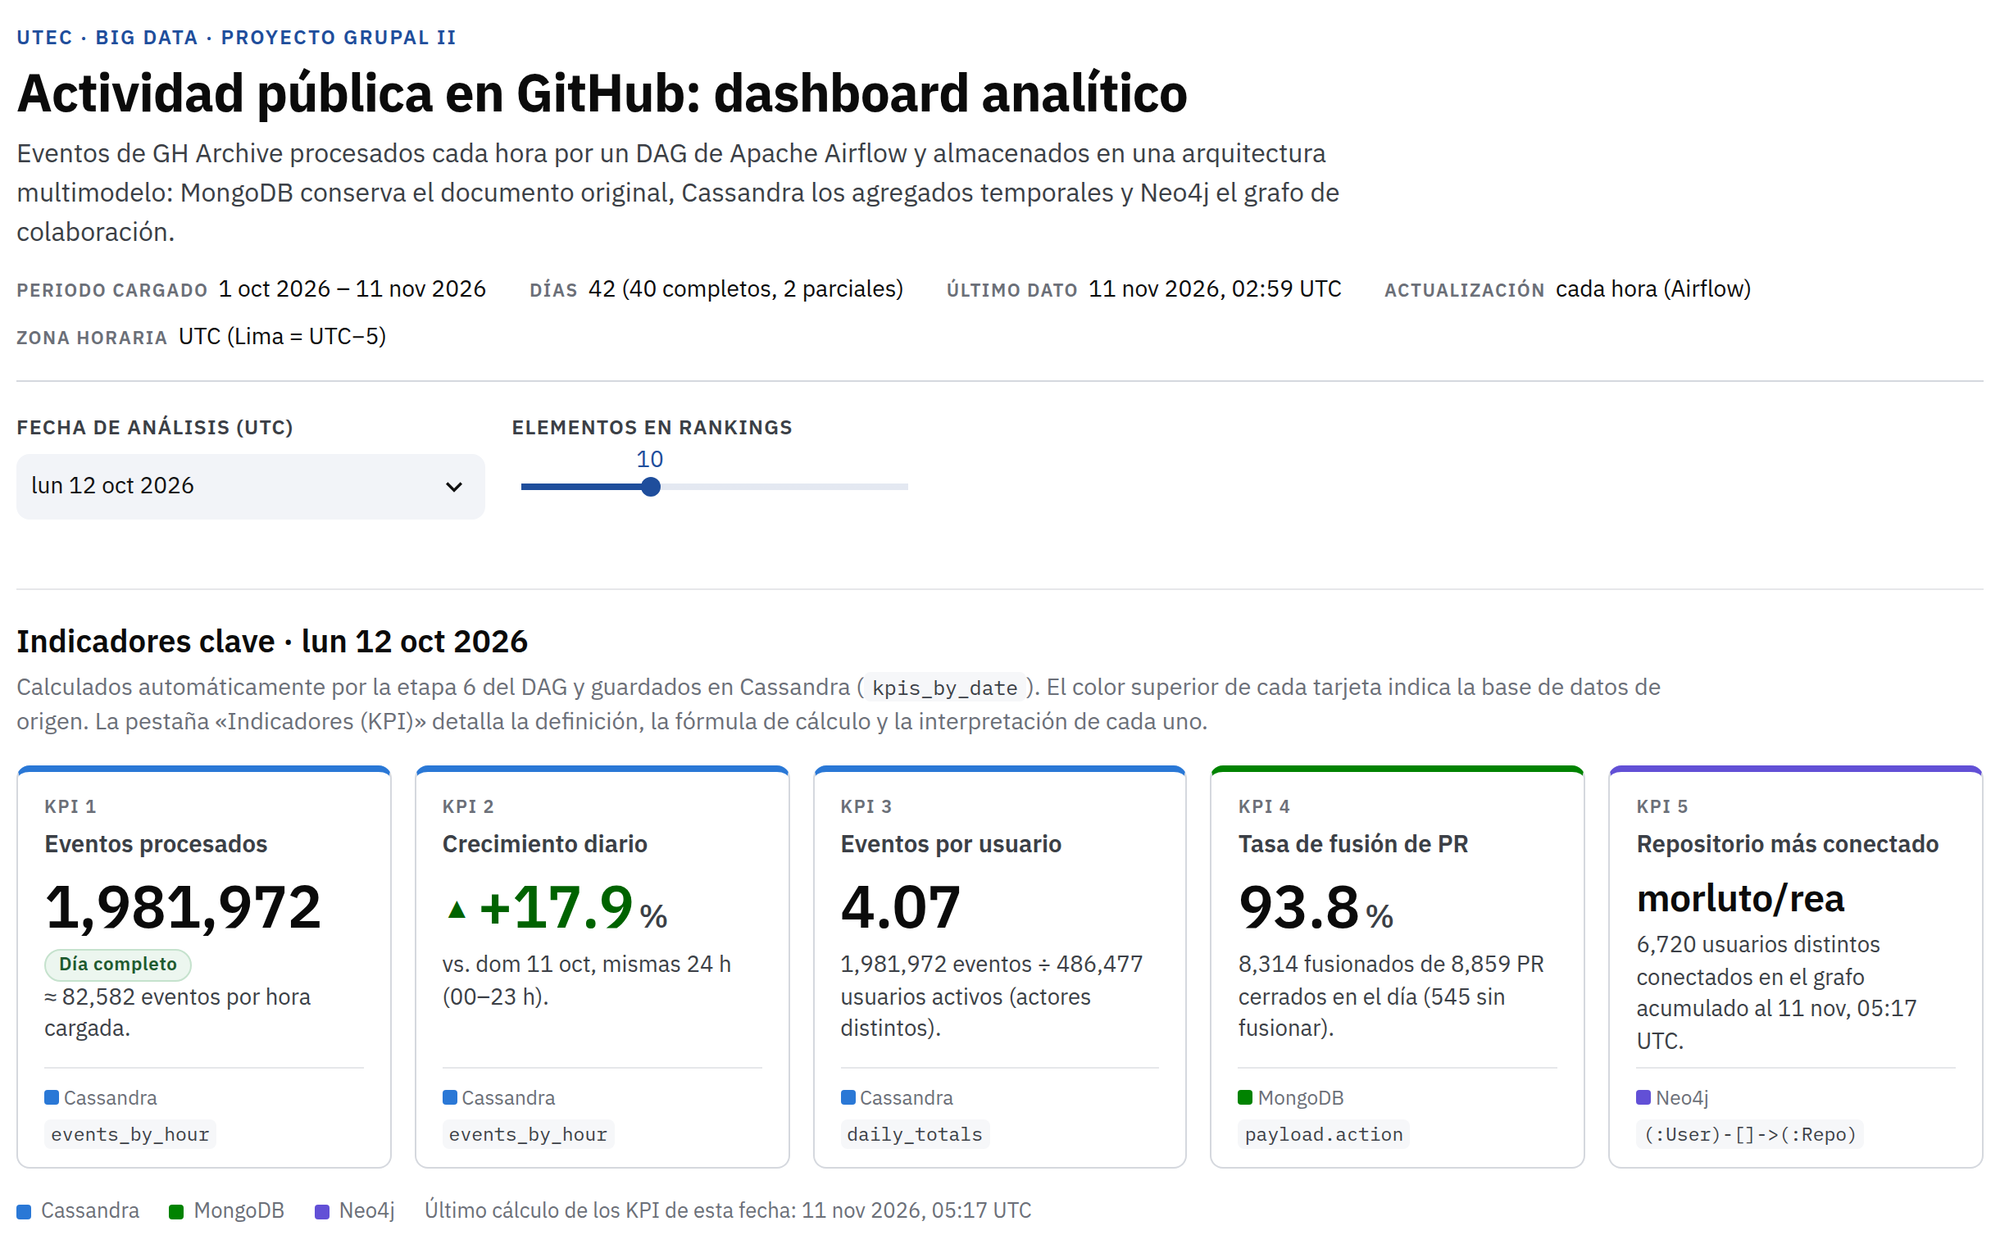
\includegraphics[width=\textwidth]{dash-encabezado.png}
    \caption{Encabezado del \textit{dashboard}: metadatos de cobertura, selector de fecha y tarjetas de los cinco KPI. El color del borde superior indica la base de datos de origen de cada indicador.}
    \label{fig:dash-encabezado}
\end{figure}

\begin{figure}[H]
    \centering
    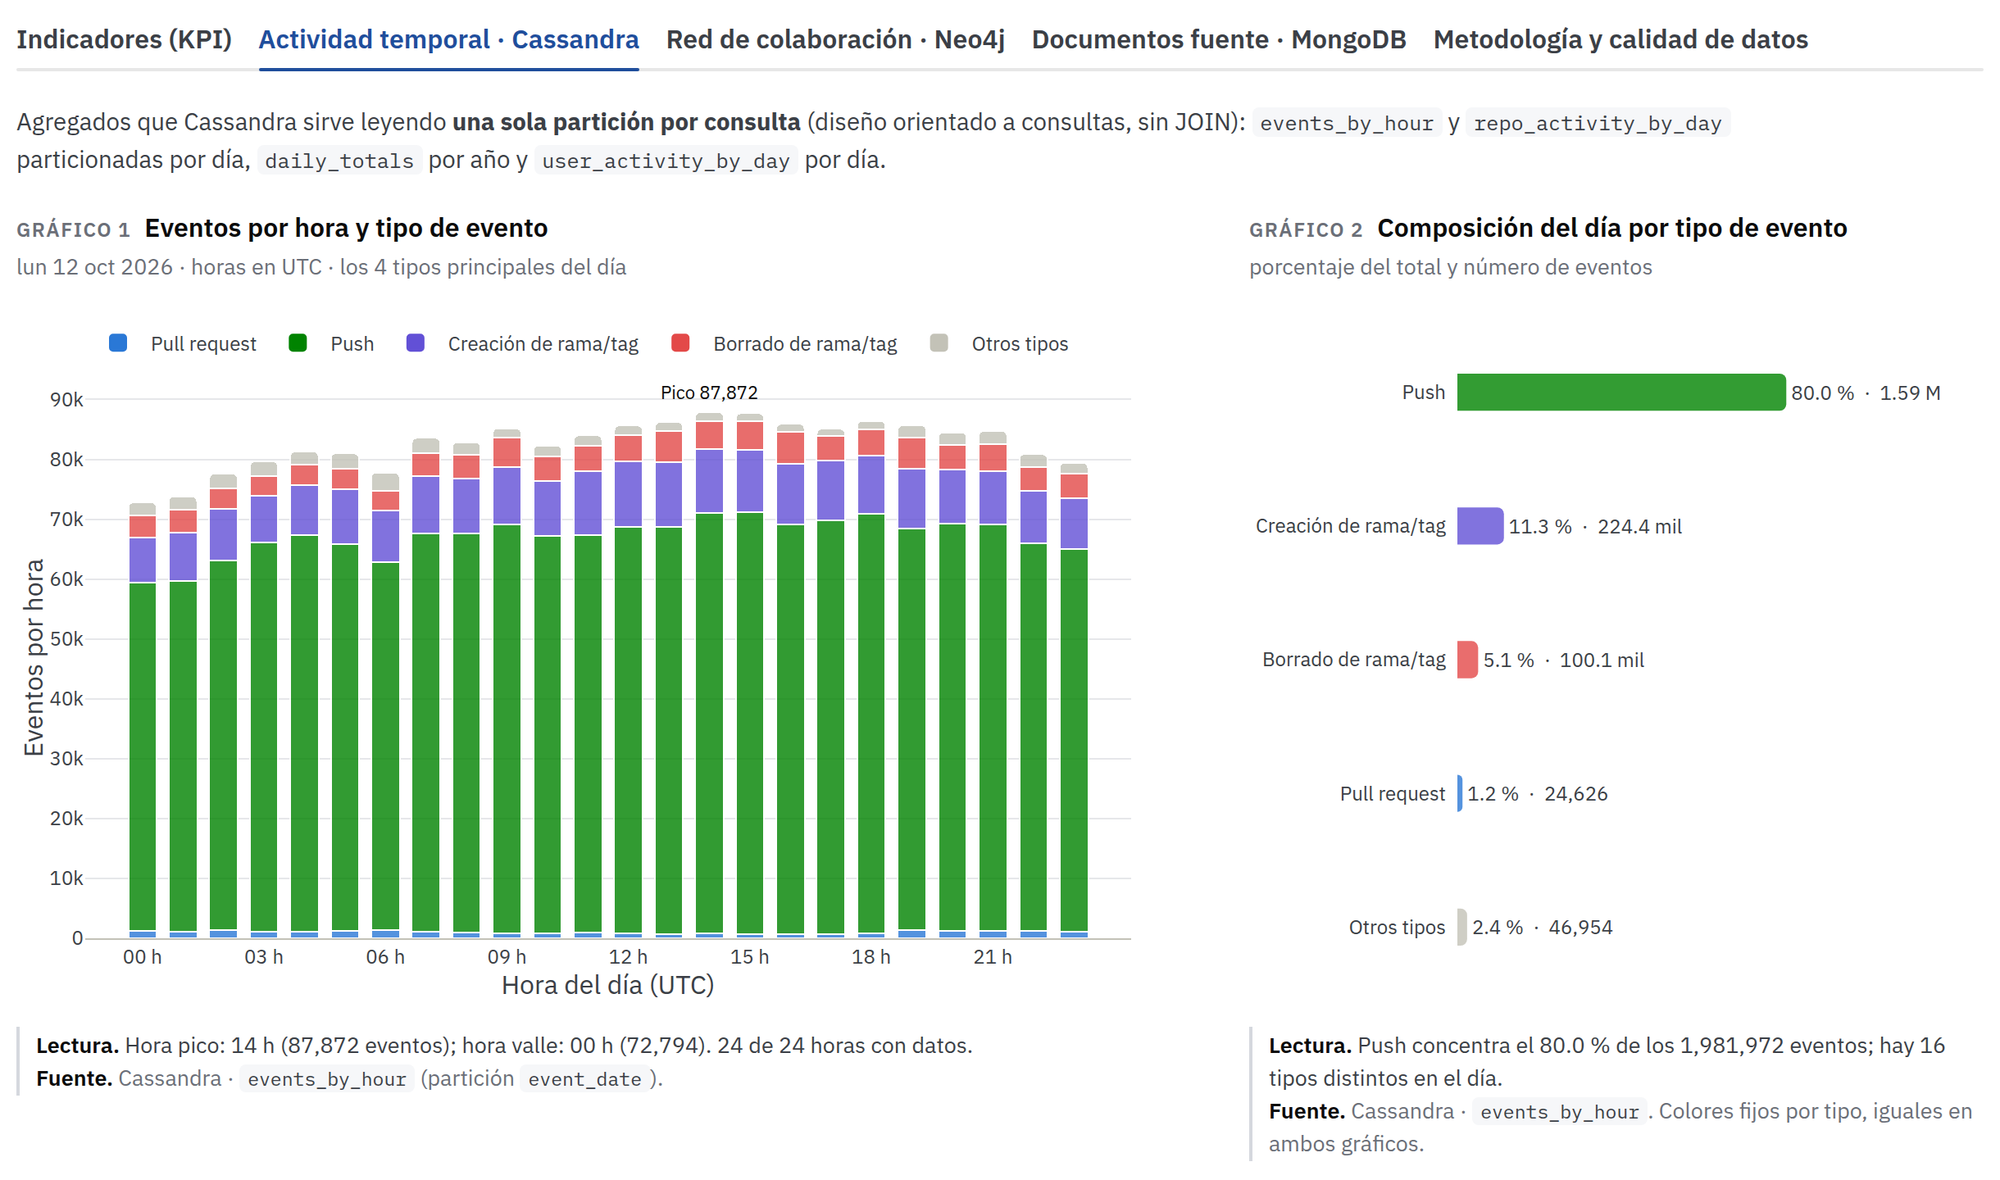
\includegraphics[width=\textwidth]{dash-cassandra-hora.png}
    \caption{Pestaña \guillemotleft{}Actividad temporal\guillemotright{} (Cassandra). Gráfico 1: eventos por hora y tipo. Gráfico 2: composición del día. Ambos se obtienen de una única partición de \texttt{events\_by\_hour}.}
    \label{fig:dash-cassandra-hora}
\end{figure}

\begin{figure}[H]
    \centering
    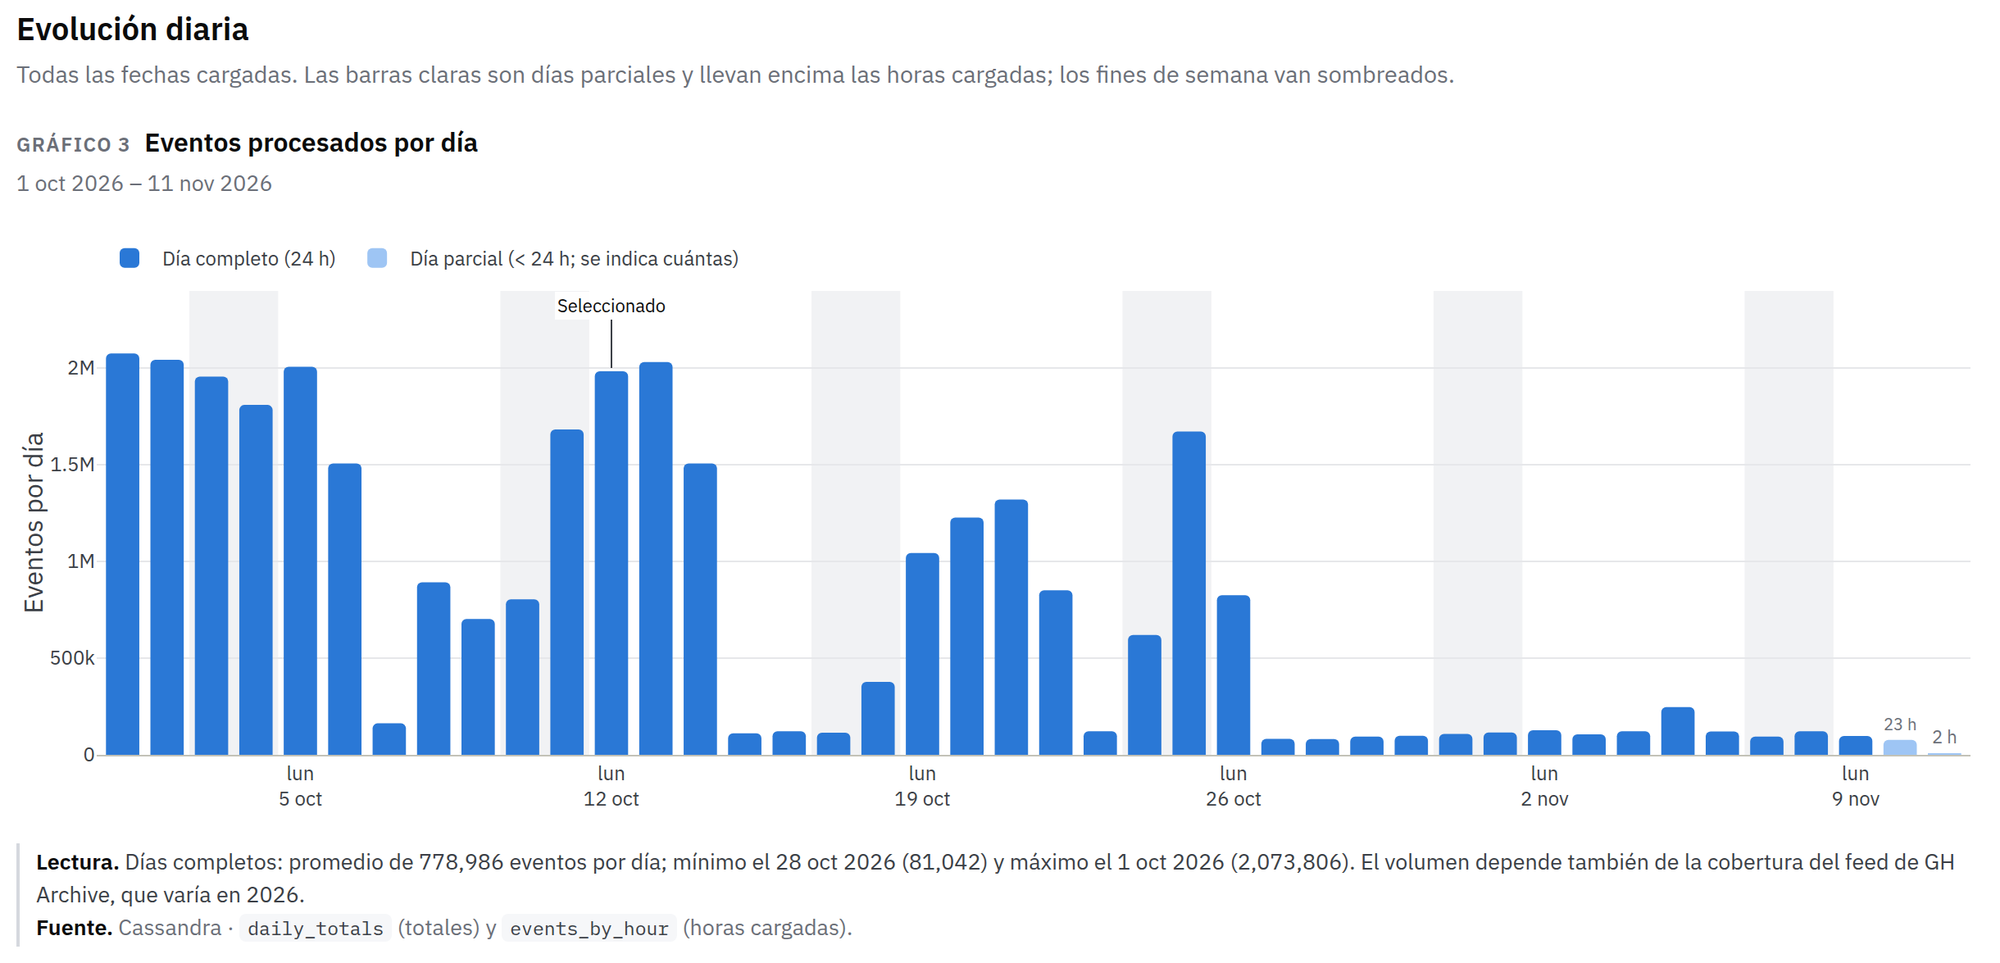
\includegraphics[width=\textwidth]{dash-cassandra-dia.png}
    \caption{Gráfico 3: eventos procesados por día en todo el periodo. Los escalones corresponden a la presencia o ausencia del flujo de referencias de Git en la fuente (Sección~\ref{subsec:cobertura}); las dos barras claras del extremo derecho son días parciales.}
    \label{fig:dash-cassandra-dia}
\end{figure}

\begin{figure}[H]
    \centering
    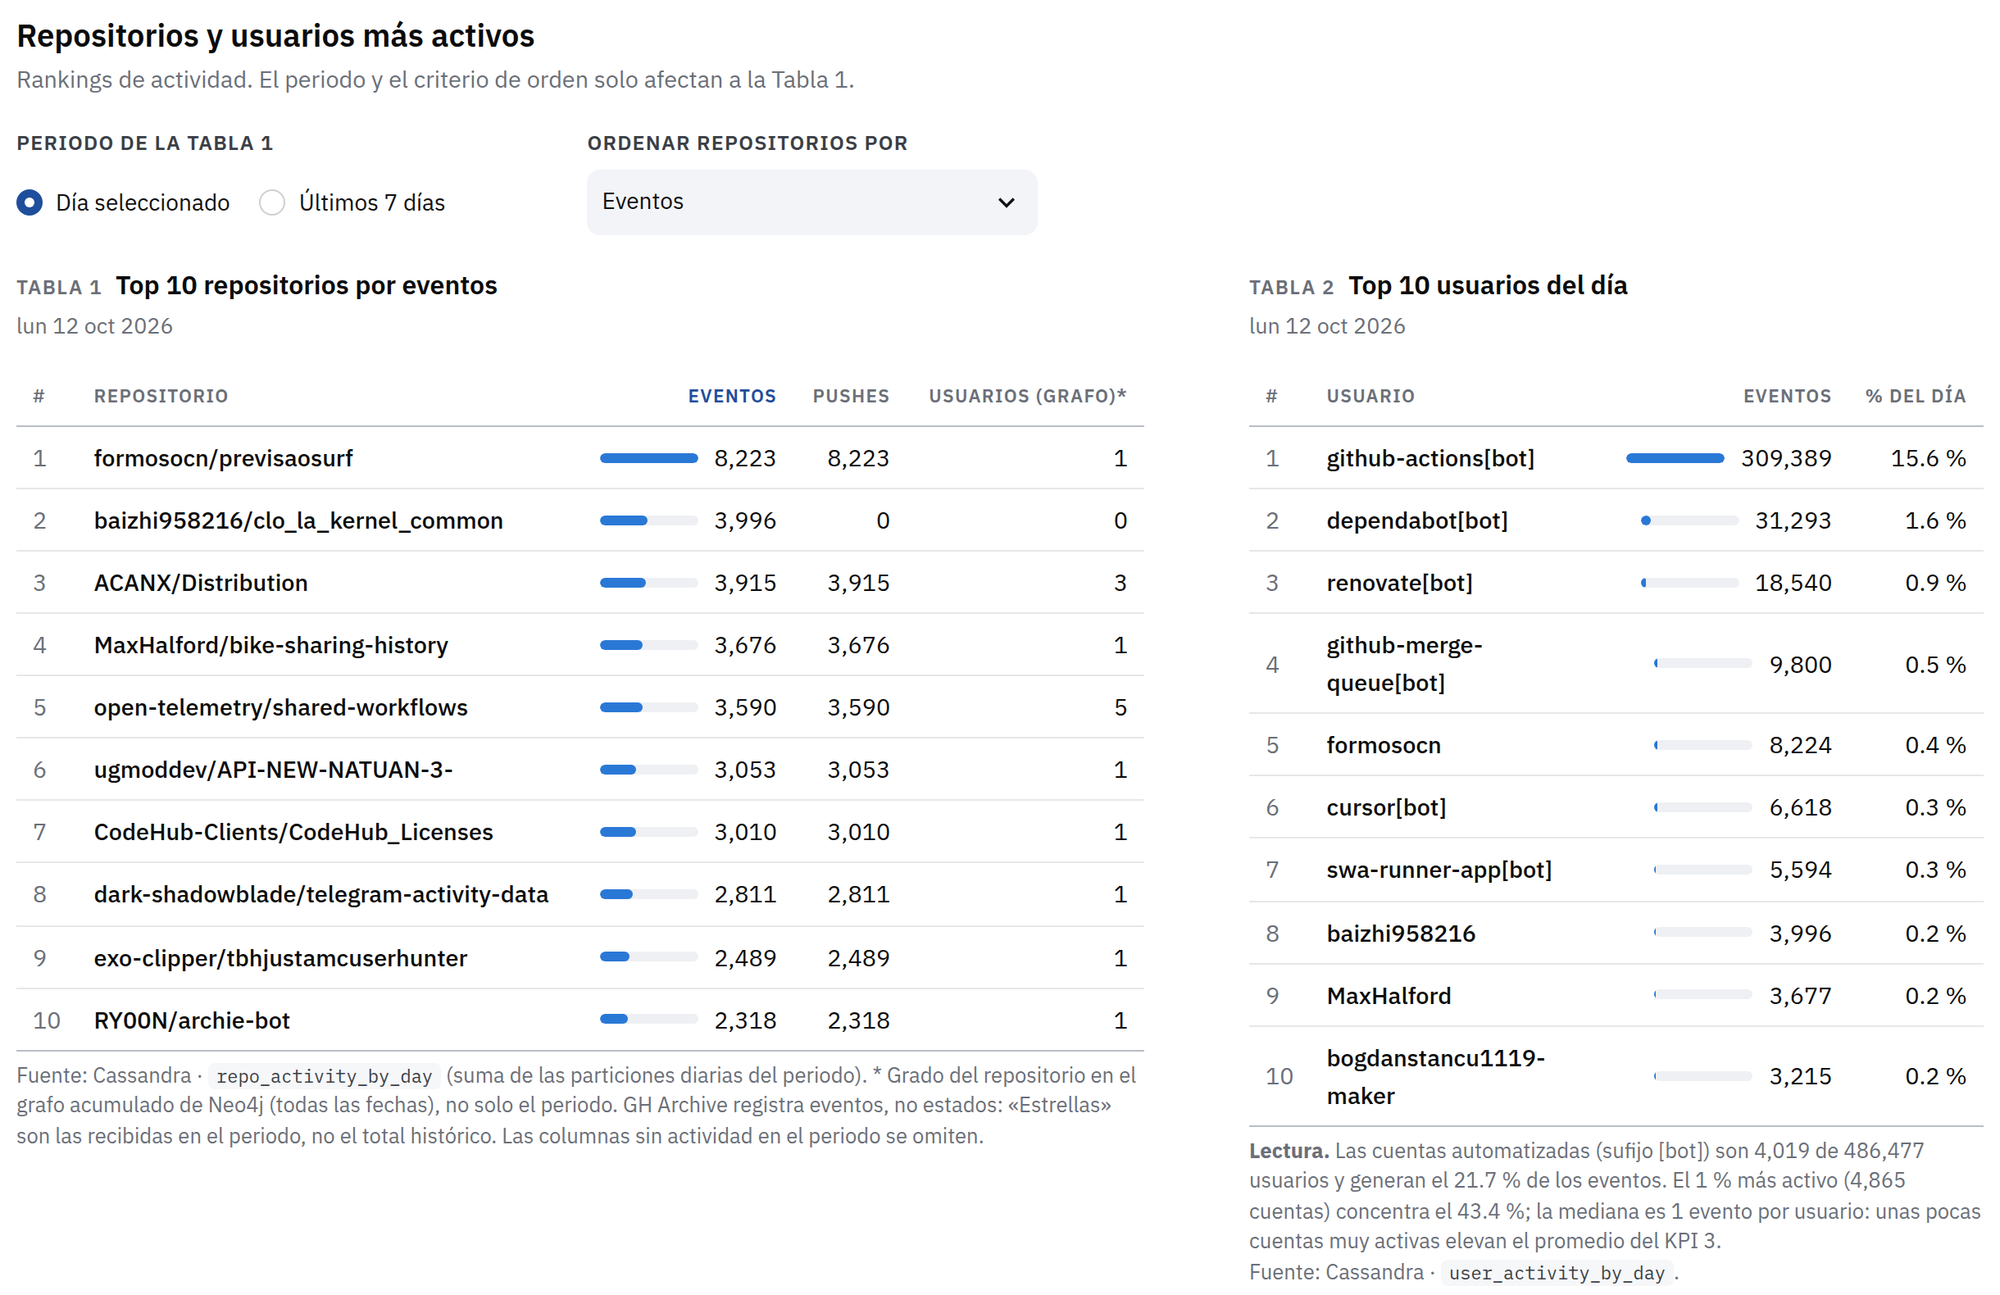
\includegraphics[width=\textwidth]{dash-cassandra-rankings.png}
    \caption{Tablas 1 y 2: repositorios y usuarios más activos del día. La columna \guillemotleft{}Usuarios (grafo)\guillemotright{} de la Tabla 1 cruza cada repositorio de Cassandra con su grado en Neo4j.}
    \label{fig:dash-cassandra-rankings}
\end{figure}

\begin{figure}[H]
    \centering
    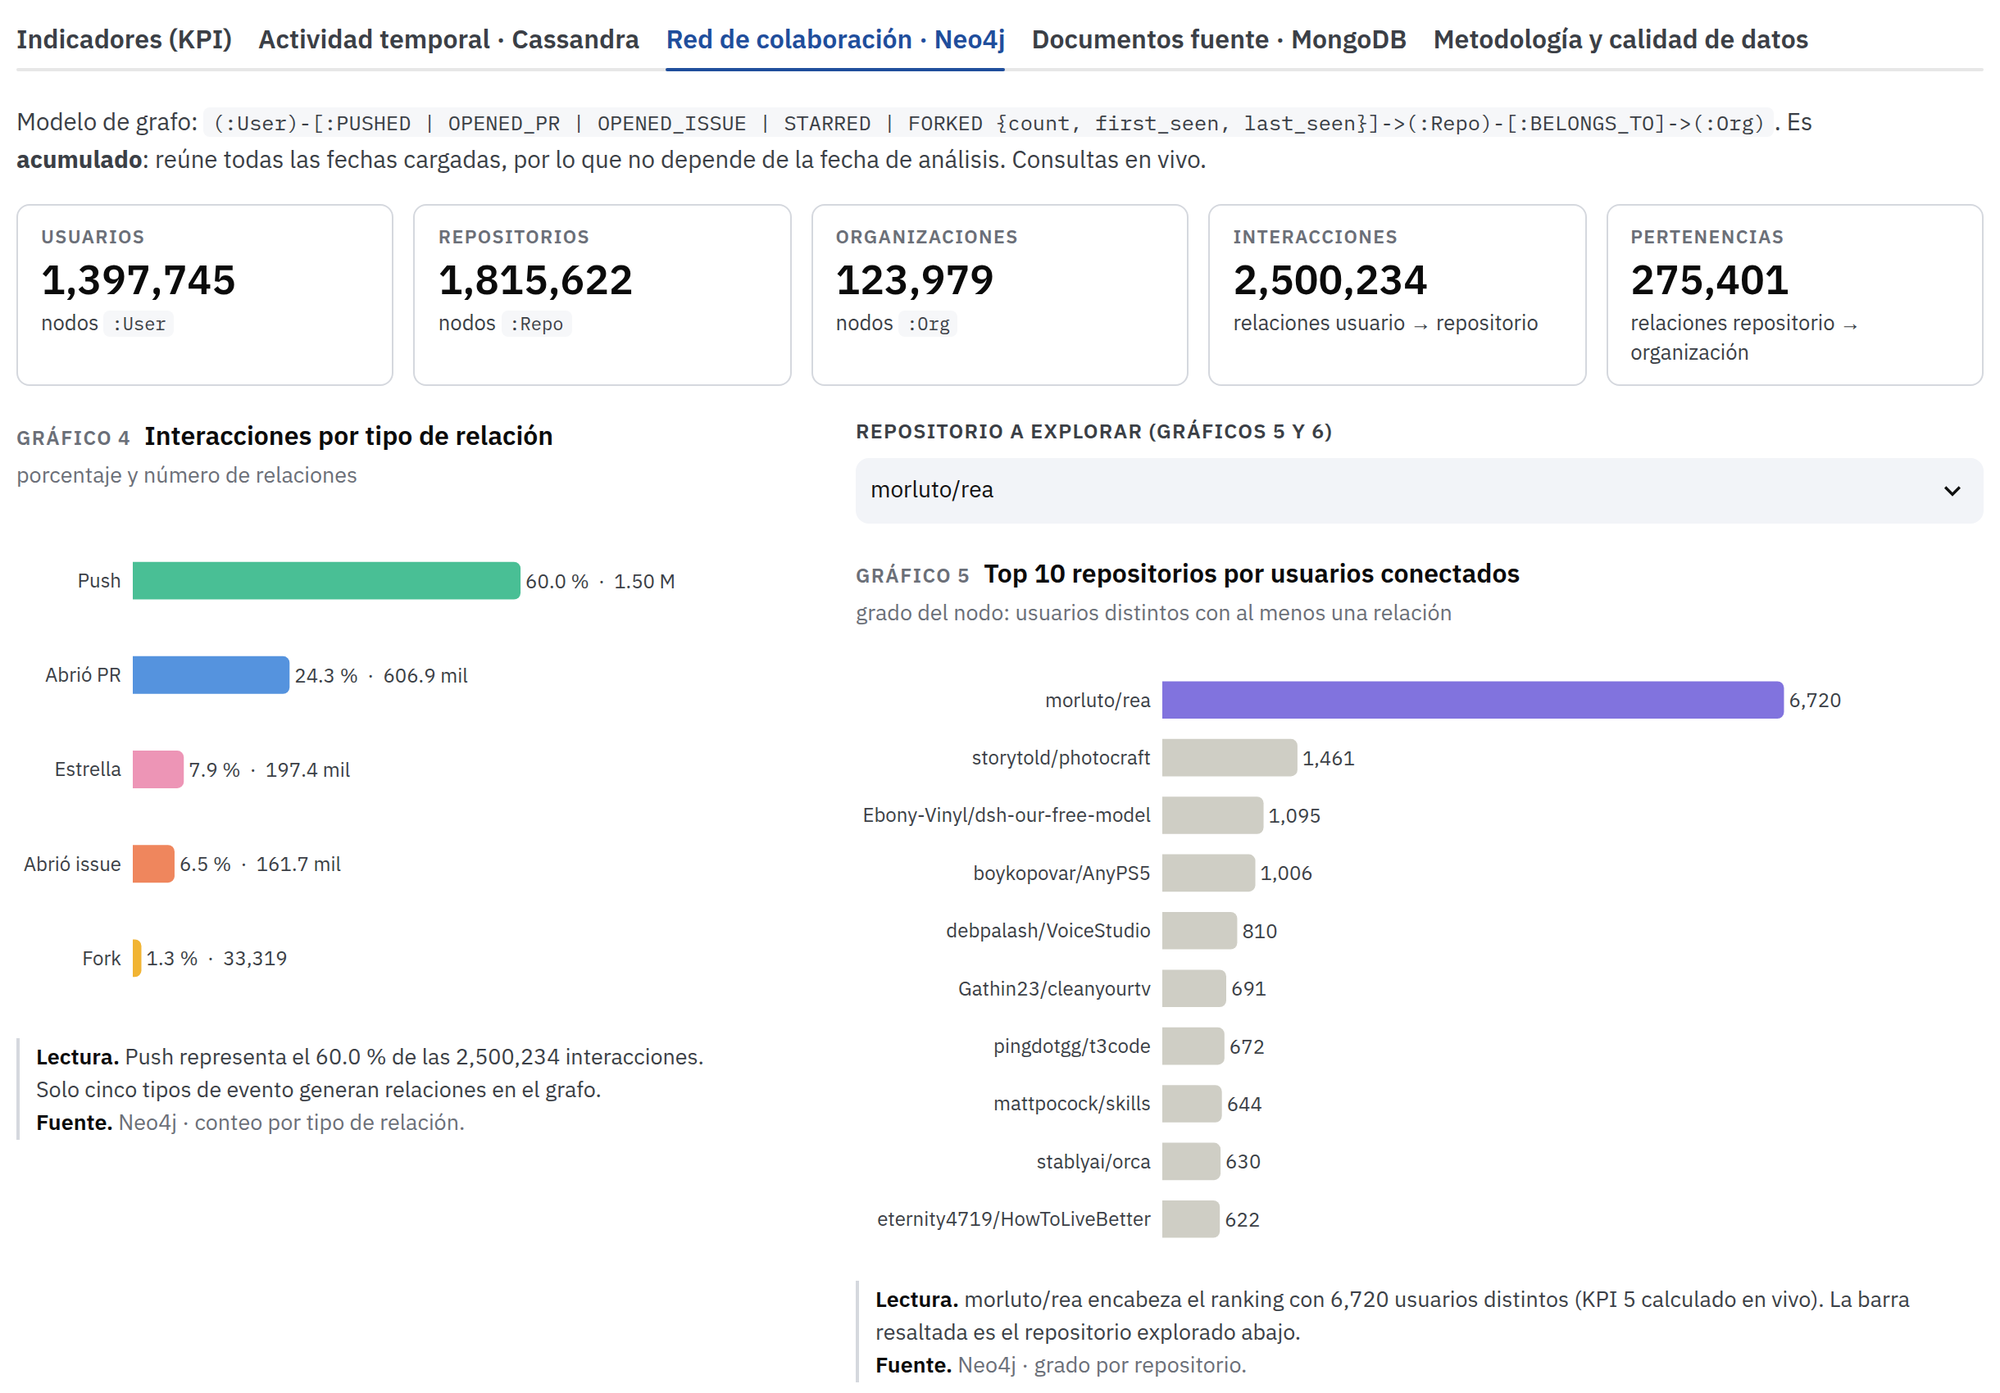
\includegraphics[width=\textwidth]{dash-neo4j-resumen.png}
    \caption{Pestaña \guillemotleft{}Red de colaboración\guillemotright{} (Neo4j). Tamaño del grafo, relaciones por tipo (Gráfico 4) y repositorios con más usuarios conectados (Gráfico 5).}
    \label{fig:dash-neo4j-resumen}
\end{figure}

\begin{figure}[H]
    \centering
    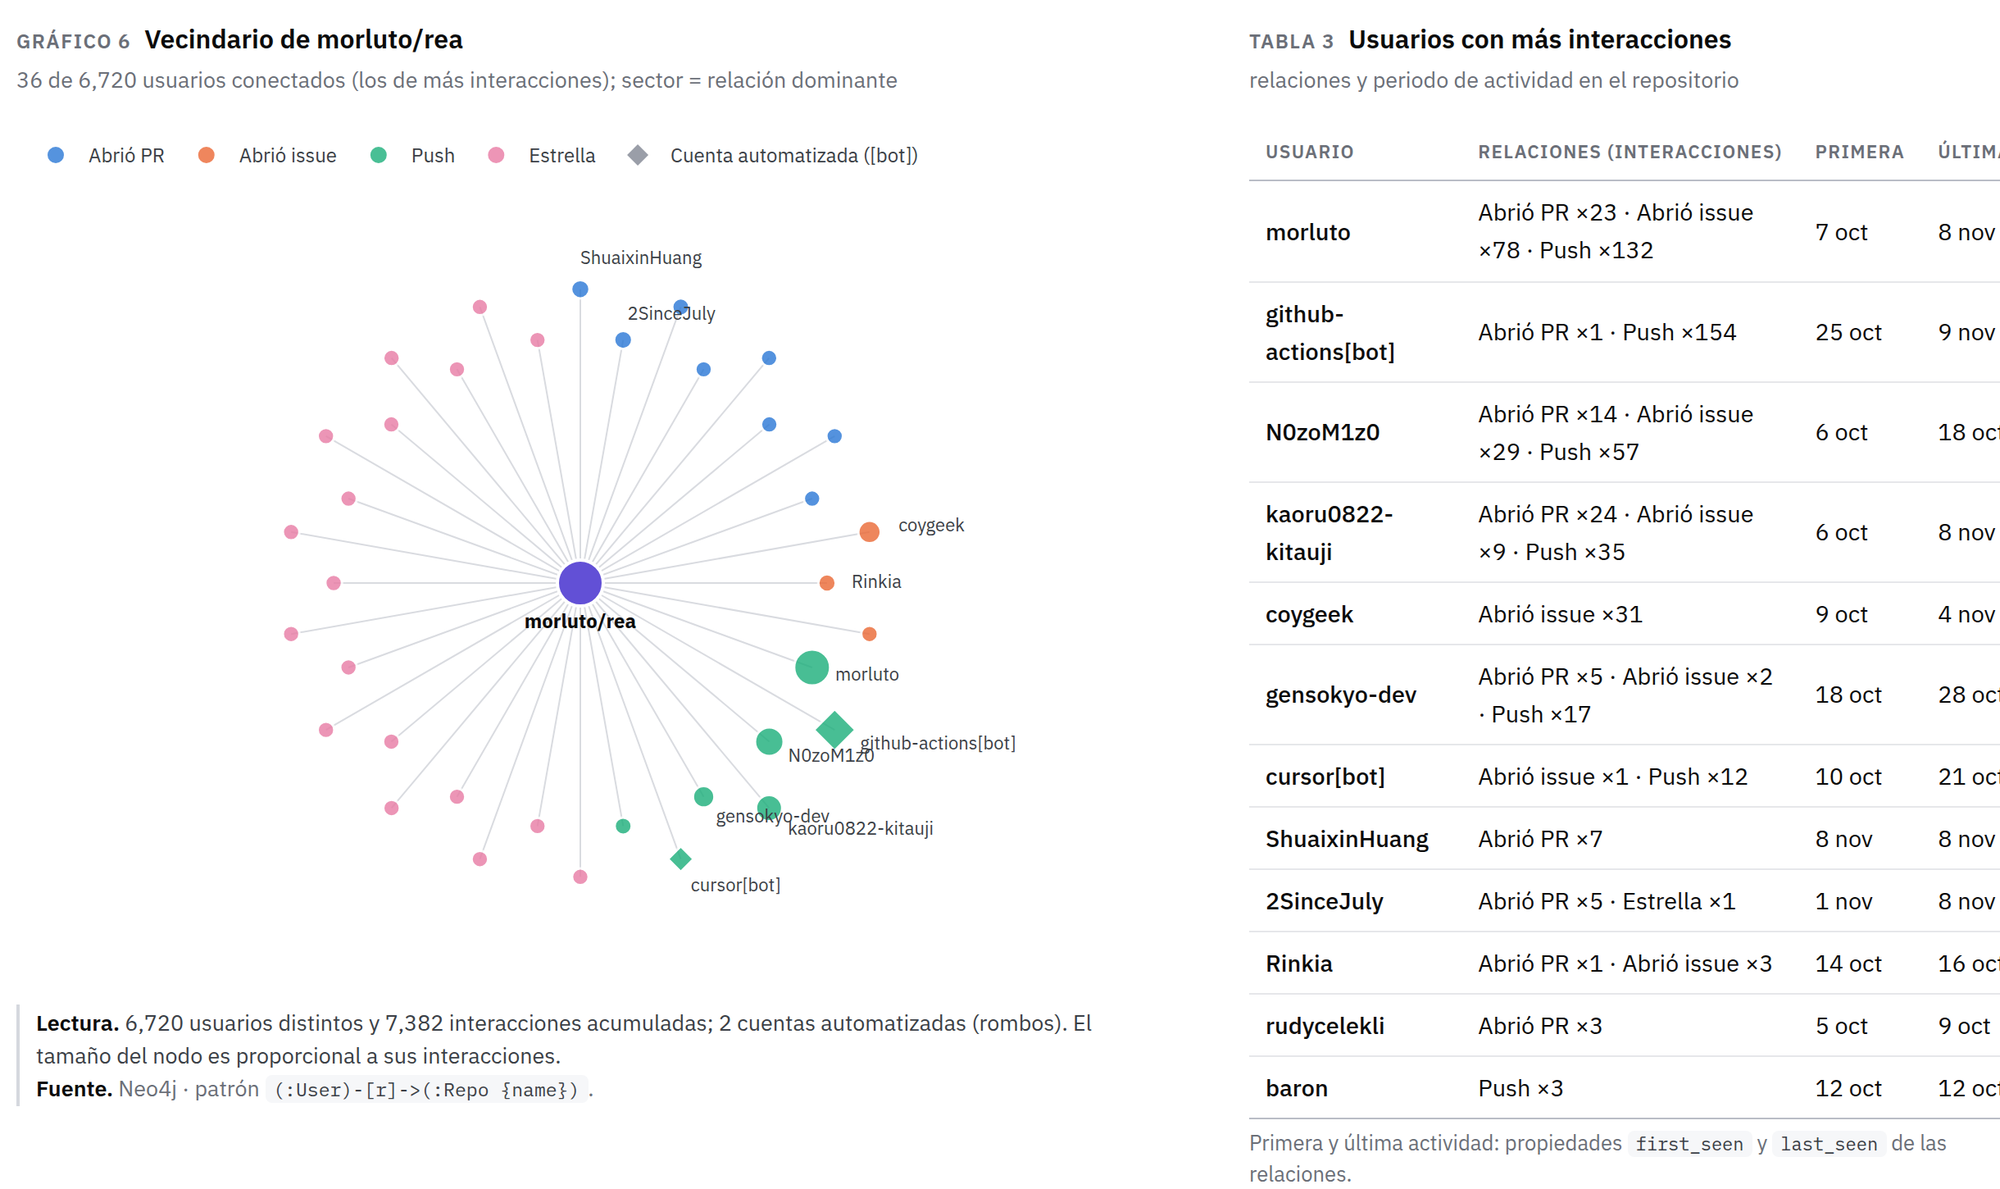
\includegraphics[width=\textwidth]{dash-neo4j-vecindario.png}
    \caption{Gráfico 6 y Tabla 3: vecindario del repositorio seleccionado. Se muestran los 36 usuarios con más interacciones; el color indica la relación dominante de cada uno y los rombos, cuentas automatizadas.}
    \label{fig:dash-neo4j-vecindario}
\end{figure}

\begin{figure}[H]
    \centering
    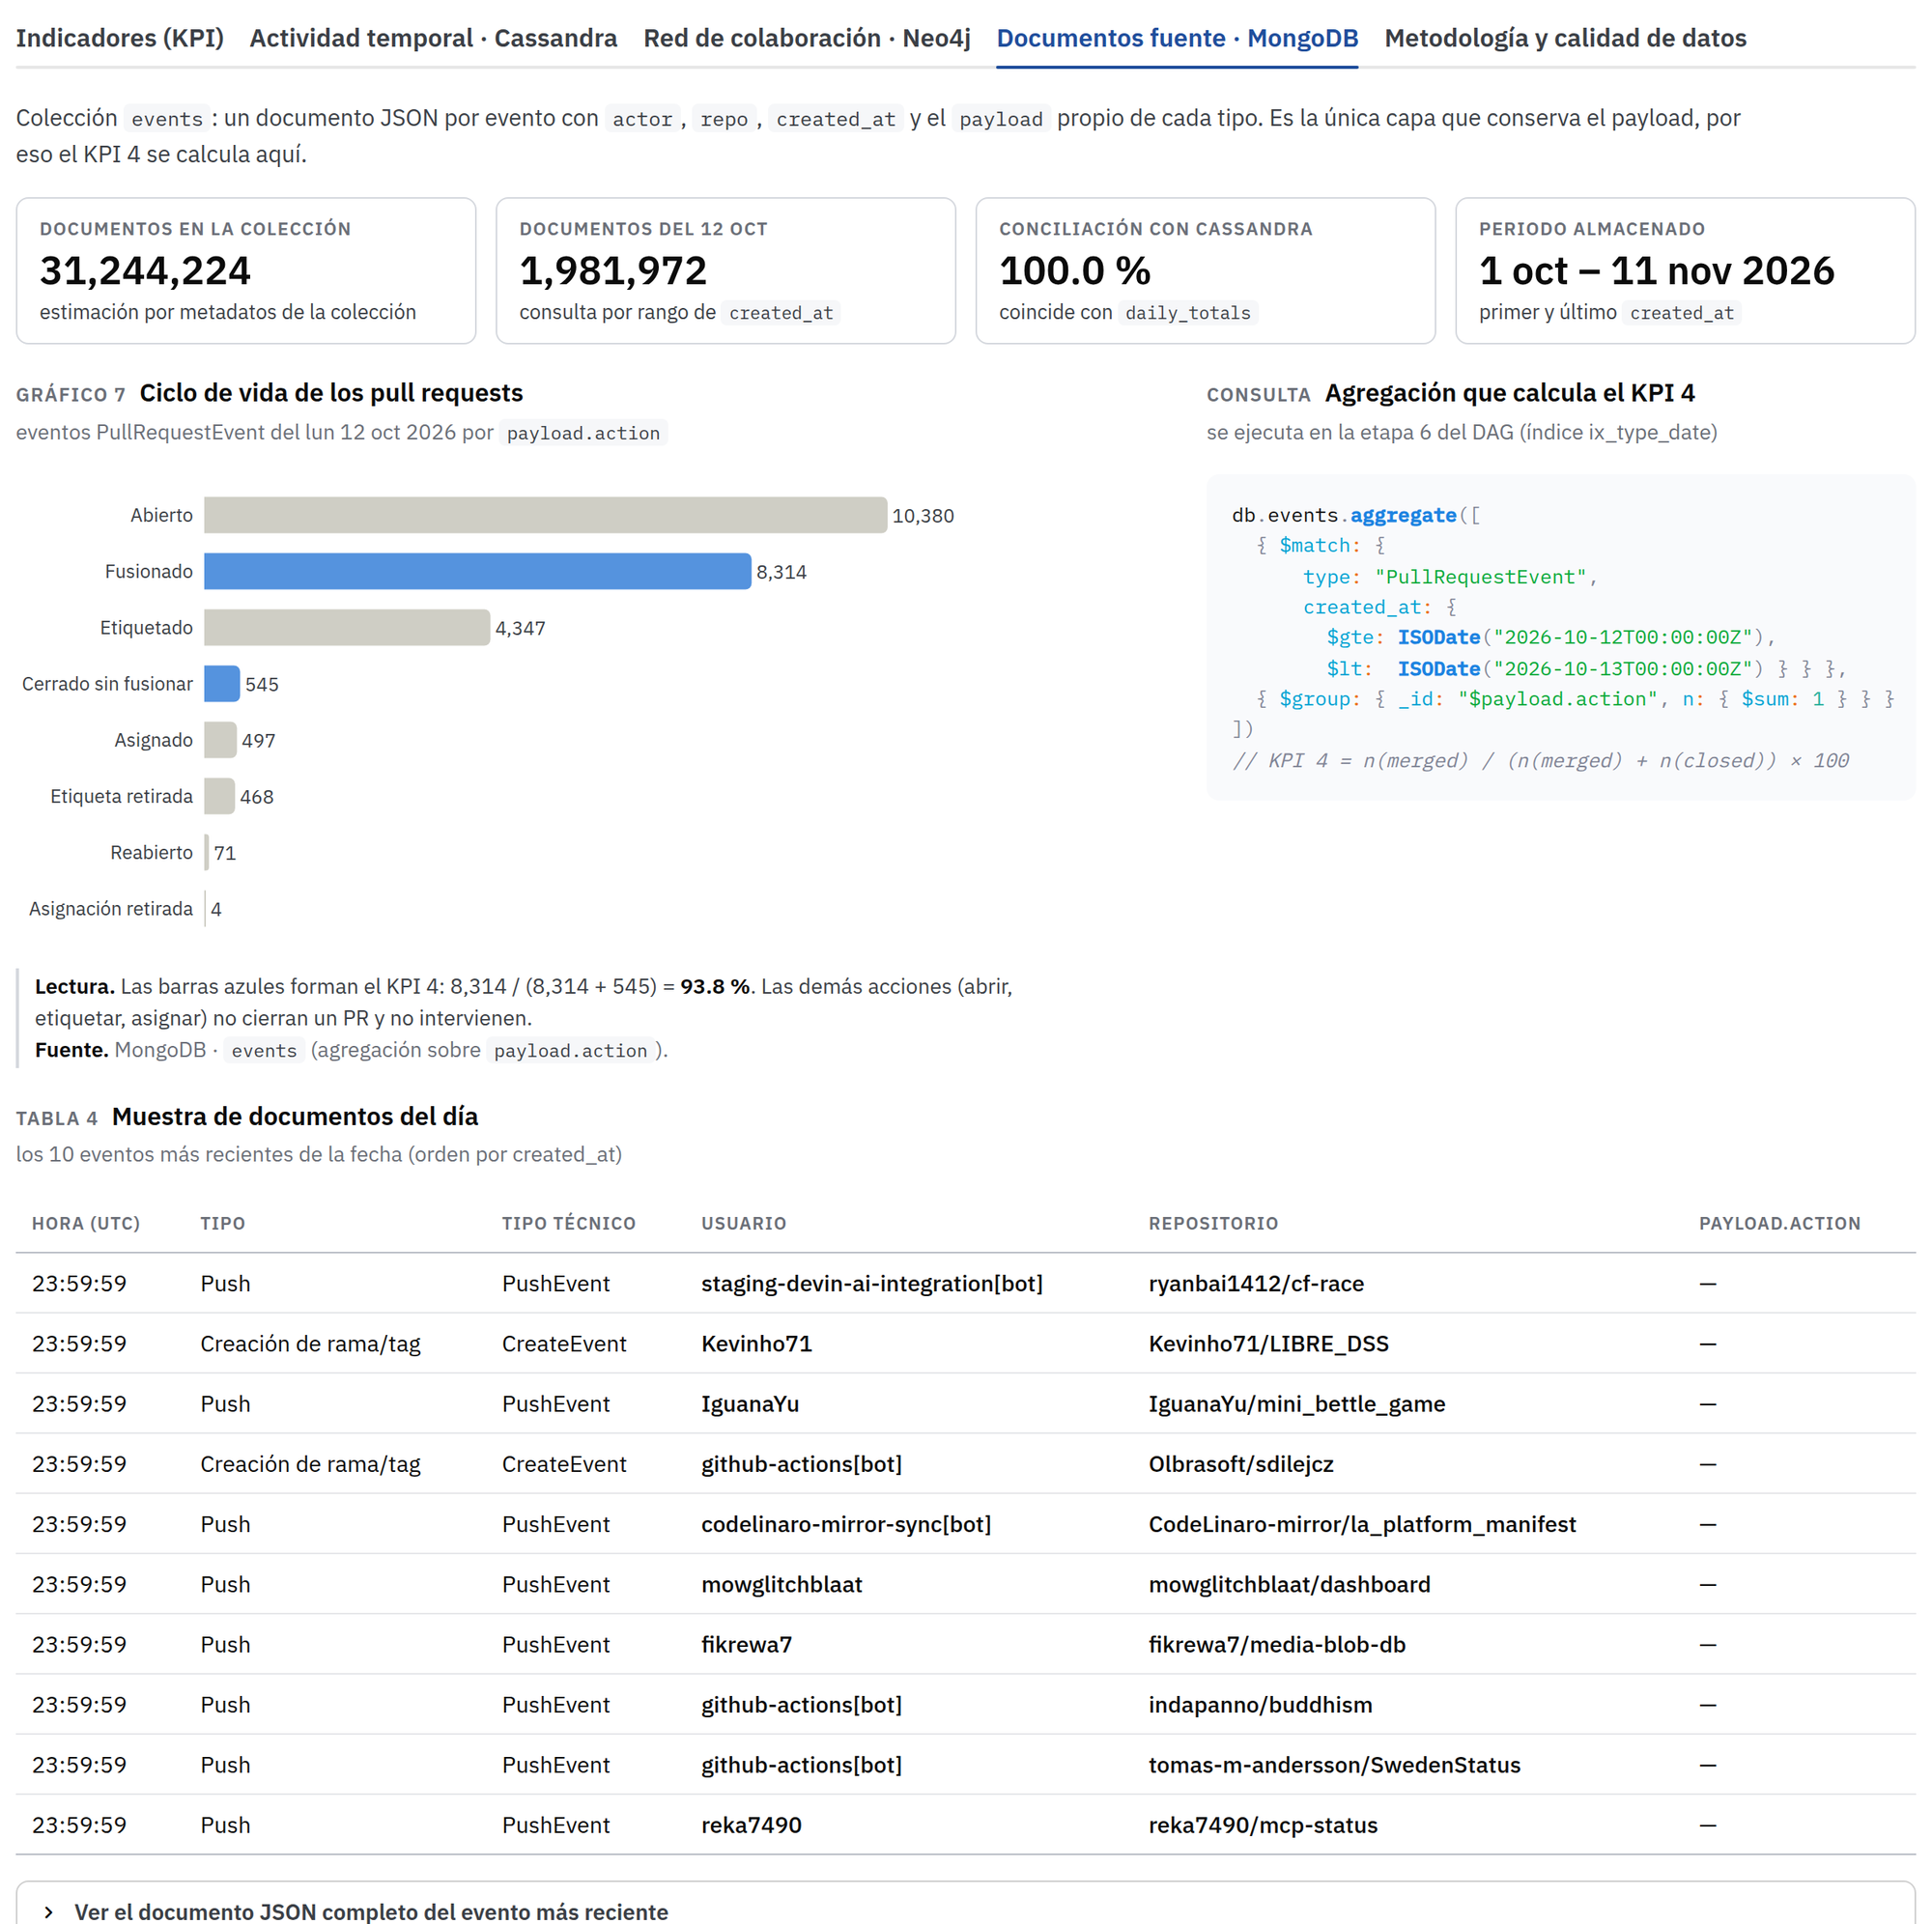
\includegraphics[width=0.96\textwidth]{dash-mongodb.png}
    \caption{Pestaña \guillemotleft{}Documentos fuente\guillemotright{} (MongoDB). La tarjeta de conciliación compara el conteo de documentos del día con el total de Cassandra (100\,\%). El Gráfico 7 muestra las acciones de los \textit{pull requests}; las dos barras resaltadas forman el KPI 4.}
    \label{fig:dash-mongodb}
\end{figure}

\begin{figure}[H]
    \centering
    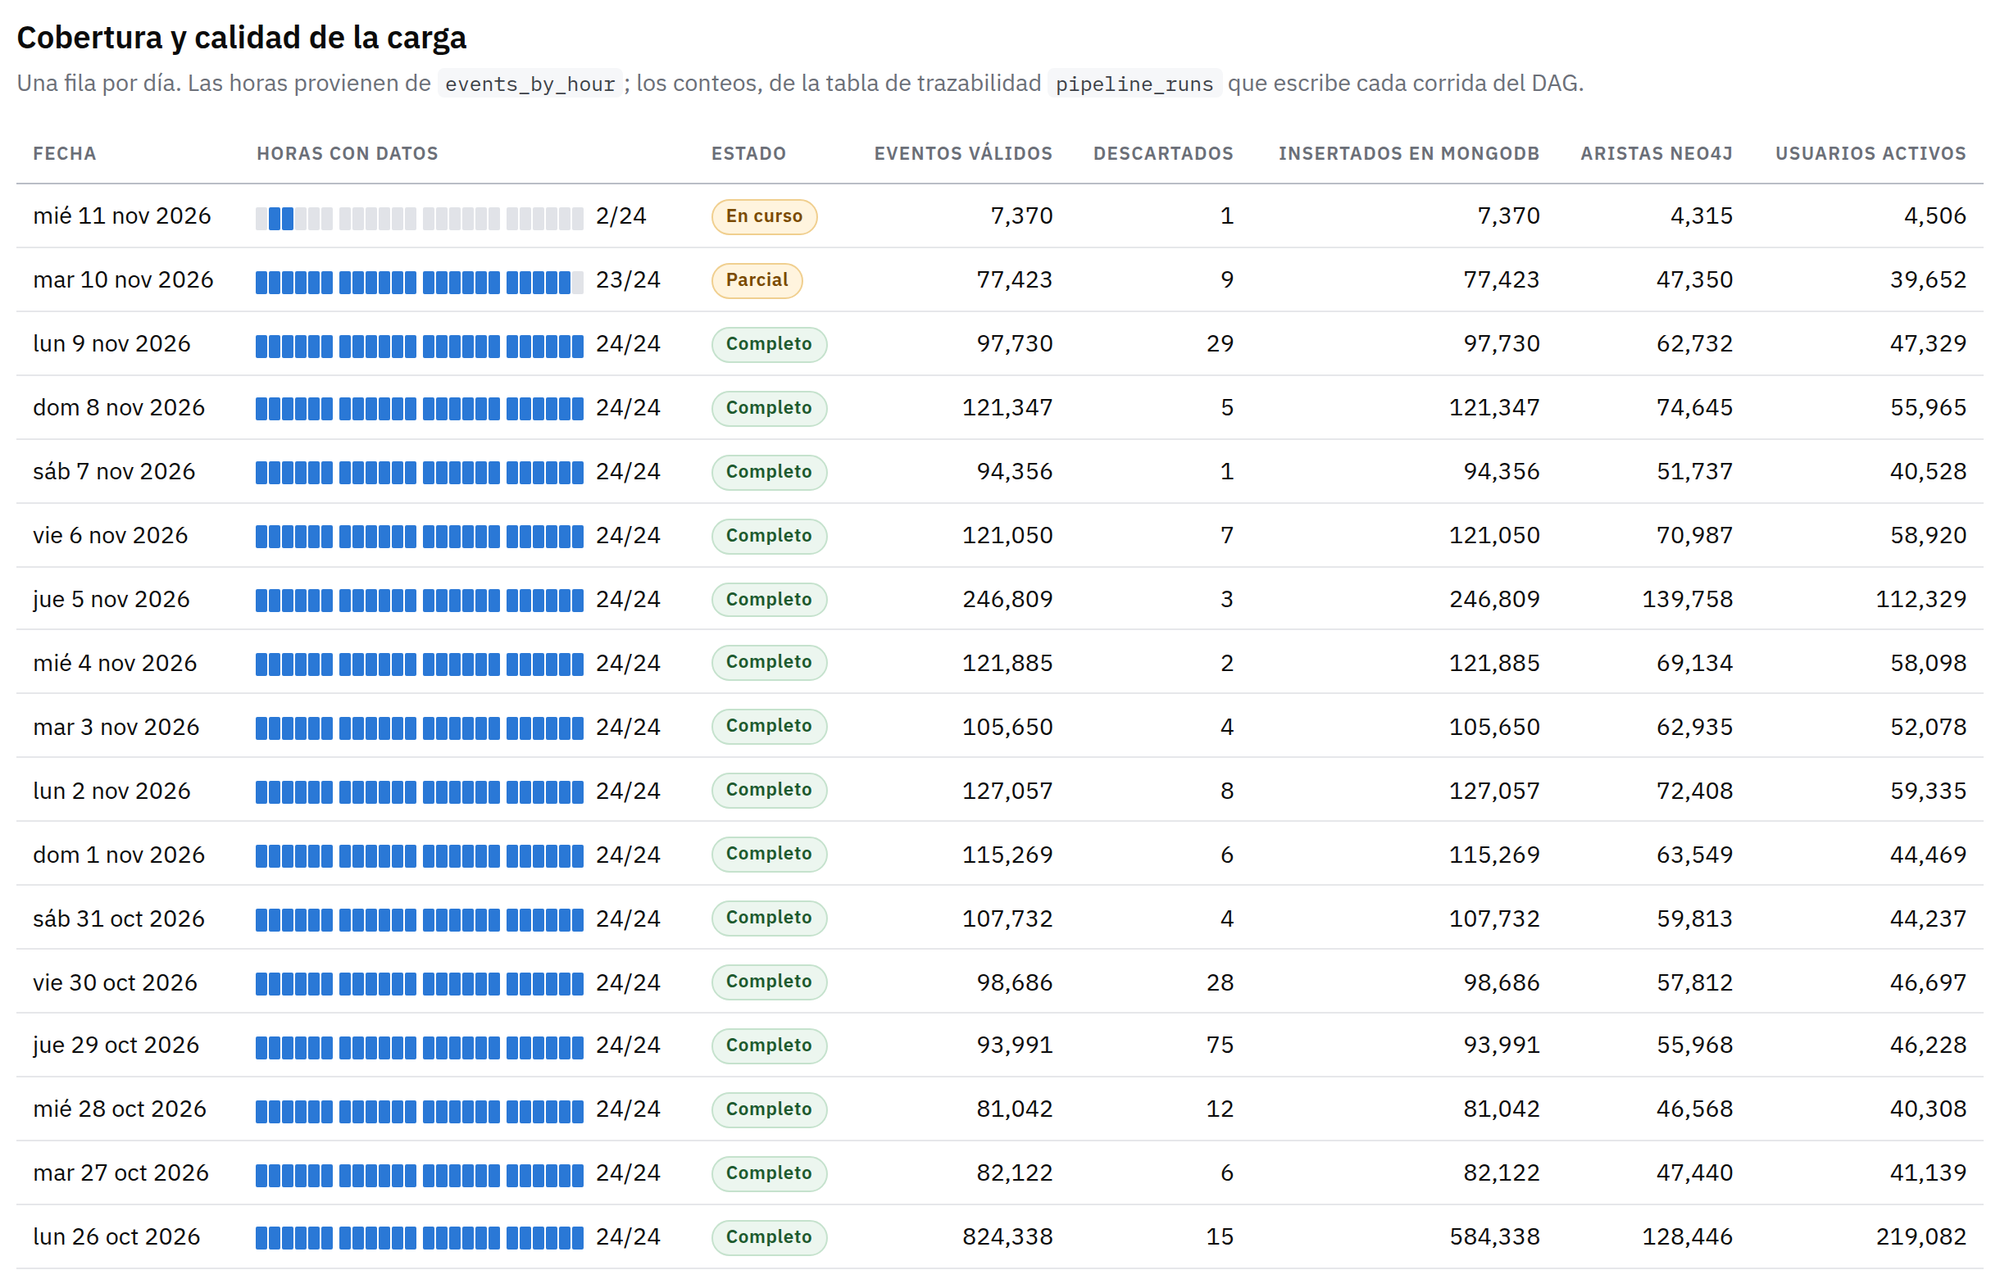
\includegraphics[width=\textwidth]{dash-cobertura.png}
    \caption{Pestaña \guillemotleft{}Metodología y calidad de datos\guillemotright{}: cobertura de la carga día por día (extracto), construida a partir de \texttt{events\_by\_hour} y de la tabla de trazabilidad \texttt{pipeline\_runs}.}
    \label{fig:dash-cobertura}
\end{figure}

\begin{figure}[H]
    \centering
    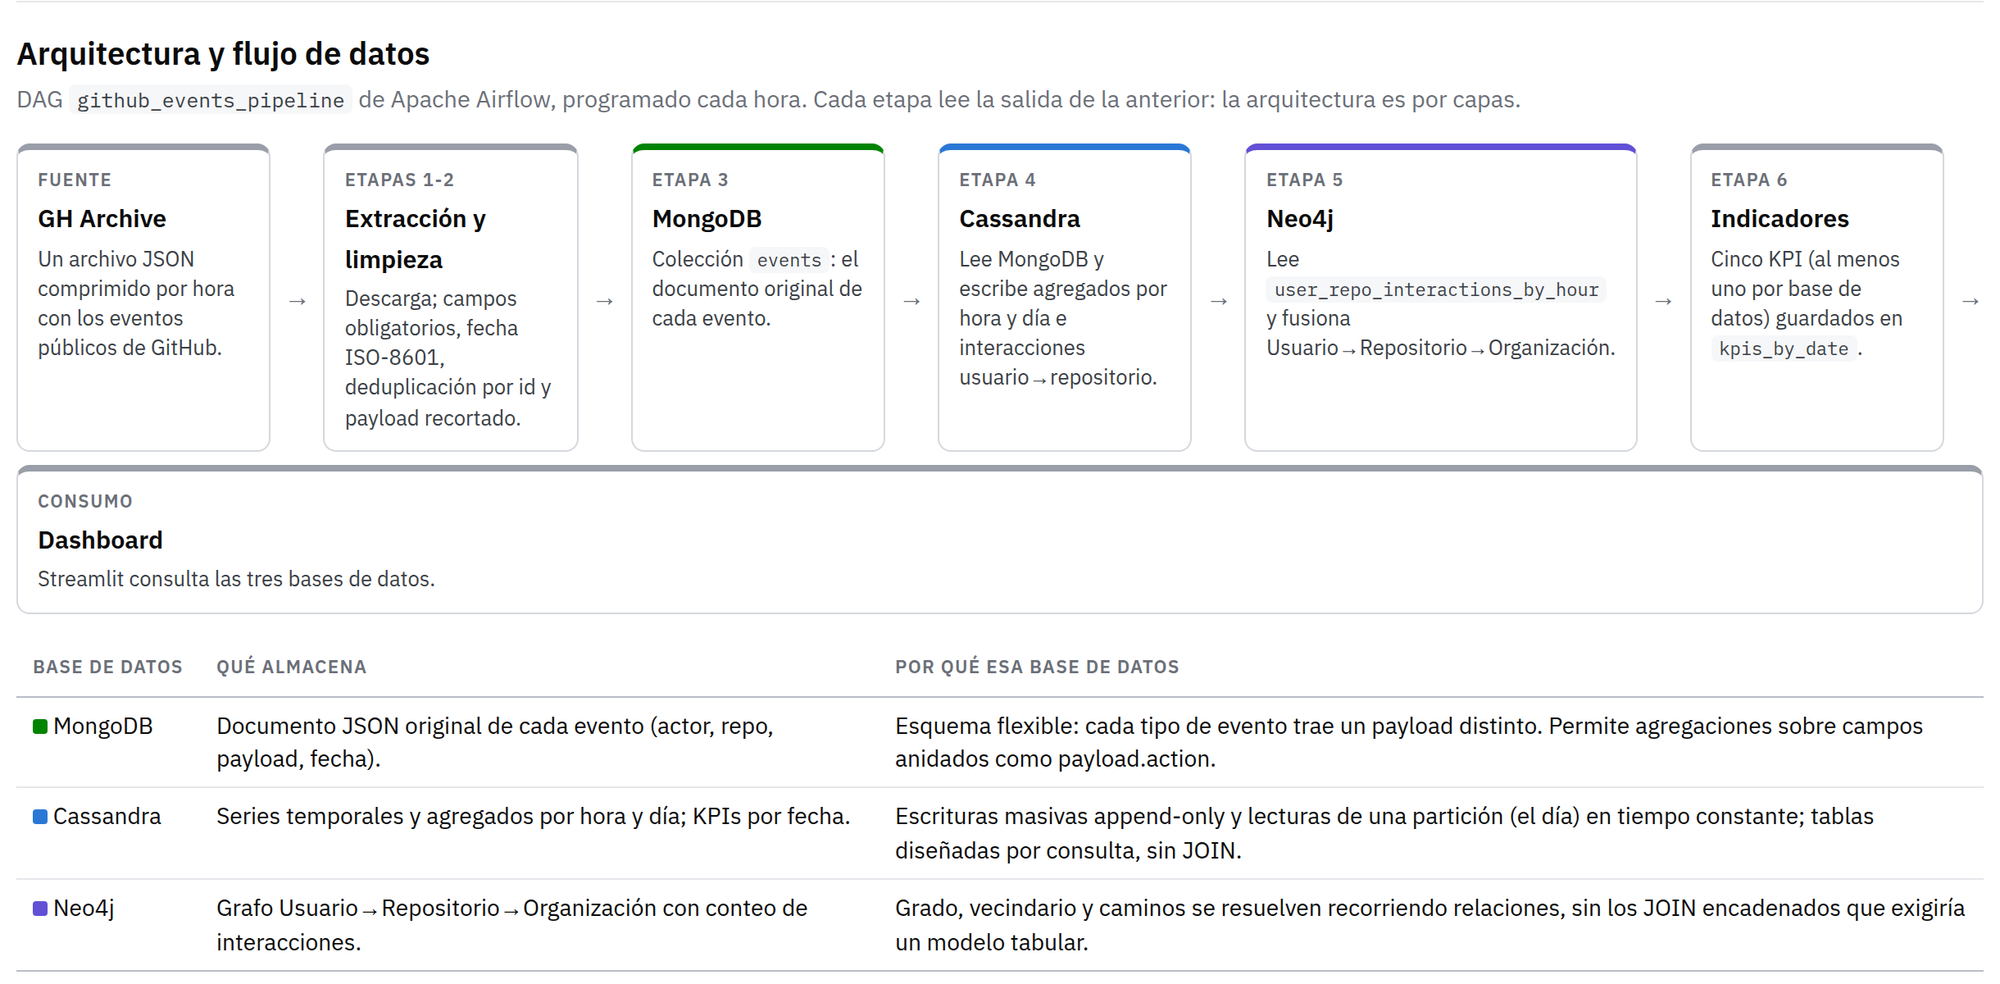
\includegraphics[width=\textwidth]{dash-arquitectura.png}
    \caption{El propio \textit{dashboard} documenta el flujo de datos y la justificación de cada base, de modo que quien lo consulta puede interpretar los indicadores sin recurrir a este informe.}
    \label{fig:dash-arquitectura}
\end{figure}

% ============================ CONCLUSIONES ===========================
\section{Conclusiones}

\paragraph{1. Cada base de datos resolvió la pregunta para la que fue elegida.} MongoDB conservó los 31.2 millones de eventos con su \texttt{payload} heterogéneo y permitió calcular el único indicador que depende de un campo anidado. Cassandra sirve los gráficos temporales desde tablas que suman menos de 1~MB, leyendo una partición por consulta. Neo4j responde preguntas de conectividad sobre 3.3 millones de nodos y 2.8 millones de relaciones. La justificación no es teórica: el KPI~4 no puede obtenerse de Cassandra, y el análisis del repositorio más conectado no puede obtenerse sin los tipos de relación del grafo.

\paragraph{2. La arquitectura por capas hizo que dos de las tres bases fueran reconstruibles.} Al alimentar Cassandra desde MongoDB y Neo4j desde Cassandra, y no las tres desde el archivo de origen, MongoDB queda como única fuente de la verdad. El grafo puede regenerarse completo sin volver a descargar ni a limpiar un solo archivo, y los indicadores se recalcularon para todo el periodo cuando cambió la definición del KPI~2. El costo es una dependencia secuencial: un fallo en una capa detiene las siguientes.

\paragraph{3. El \textit{pipeline} no pierde datos, y se comprobó en lugar de suponerlo.} Una auditoría independiente sobre los 985 archivos de origen contó 31,244,816 eventos crudos, de los cuales 190 se rechazan por validación y 402 por duplicados. Los 31,244,224 restantes coinciden exactamente con el número de documentos en MongoDB. Ninguna hora alcanzó el tope de eventos y ningún archivo contenía JSON inválido.

\paragraph{4. El principal hallazgo del proyecto es sobre la fuente, no sobre GitHub.} El volumen de los días completos varía en un factor de 25.6, pero esa variación no describe la actividad de la plataforma. Los eventos \texttt{PushEvent}, \texttt{CreateEvent} y \texttt{DeleteEvent}, que suman el 85.9\,\% del dataset, están presentes en 505 archivos horarios y ausentes en los otros 480, siempre los tres a la vez; el resto de los tipos se mantiene estable en todo el periodo. Los días con ese flujo completo promedian 1.74 millones de eventos y los días sin él, 108 mil. Un tablero que presentara el volumen diario como \guillemotleft{}tendencia de actividad\guillemotright{} estaría midiendo la cobertura del colector de GH Archive.

\paragraph{5. Un indicador solo es útil si se conoce qué mide.} La consecuencia práctica del punto anterior es que los KPI~1 y~2 no son comparables entre días con distinta cobertura, mientras que el KPI~4, apoyado en el flujo estable, se mantuvo entre 88.8\,\% y 94.7\,\% durante las seis semanas. De forma análoga, el promedio de 4.07 eventos por usuario convive con una mediana de 1, porque el 1\,\% de las cuentas genera el 43.4\,\% de la actividad y las cuentas automatizadas, el 21.7\,\%. Por eso el \textit{dashboard} acompaña cada gráfico con su lectura y declara sus limitaciones.

\paragraph{6. Un grado alto en el grafo no equivale a una comunidad.} El repositorio más conectado reúne 6,720 usuarios, cuatro veces más que el segundo, pero el 82\,\% de ellos solo le dio una estrella y apenas 7 cuentas hicieron \textit{push}. El modelo de grafo, al conservar el tipo de cada relación, permitió distinguir popularidad de colaboración; un simple conteo de usuarios por repositorio no lo habría hecho.

\paragraph{7. La idempotencia fue el requisito de ingeniería más exigente.} Cada base la resuelve de forma distinta: clave natural con \textit{upsert} en MongoDB, registro de horas procesadas en Cassandra, y la combinación de \texttt{MERGE} con ese mismo registro en Neo4j, porque \texttt{MERGE} evita duplicar aristas pero no evita sumar dos veces un contador. La limitación que subsiste está identificada: una escritura interrumpida a mitad de una hora puede acumular dos veces en las tablas diarias de Cassandra, y su remedio es recargar el día desde MongoDB.

\paragraph{8. Los fallos de operación no vinieron de los datos.} La única corrida fallida de Airflow se debió a un conflicto de permisos entre dos contenedores que comparten una carpeta, y se corrigió con una escritura atómica. Las dos horas que faltan en el registro corresponden a un intervalo en que el planificador no estuvo activo, que \texttt{catchup=False} no repone. En ambos casos el diagnóstico salió de los registros y de la tabla de trazabilidad \texttt{pipeline\_runs}, no del estado final de la corrida, la misma lección que dejó la primera entrega con los contadores de MapReduce.

\paragraph{9. Recomendaciones.} (a) Para análisis de volumen sobre este periodo conviene excluir el flujo de referencias de Git y trabajar con el flujo de colaboración, que es comparable entre días; el reporte público consultado menciona además un archivo alternativo compatible, mantenido por OpenDigger, que podría evaluarse como fuente. (b) El KPI~5 debería filtrarse por la propiedad \texttt{first\_seen} para depender de la fecha, como los otros cuatro. (c) Activar \texttt{catchup} acotado, o un sensor de horas faltantes sobre \texttt{pipeline\_runs}, haría que el sistema recupere por sí solo los intervalos en que el planificador se detiene. (d) Sustituir la acumulación por lectura y reescritura en Cassandra por columnas de tipo contador, o por el recálculo del día desde MongoDB, eliminaría la limitación de idempotencia descrita.


\end{document}
